%%%%SOLO ESTA LA HOJA 71-APROX%%%%%%%%%%%
%%REVISAR LOGARITMOS, HUBO errores%%%%%%%%%%%%%

{\sage}, ya que es un  manipulador simb\'olico, es capaz de manejar
s\'{\i}mbolos
como $\sqrt{2}$, $e$ o $\pi$, sin \lq\lq cometer ning\'un error de
aproximaci\'on\rq\rq. Pero en ocasiones deseamos tener un valor aproximado (una
expresi\'on decimal finita) de las cantidades simb\'olicas que manejamos. Esto
se puede conseguir de forma sencilla por medio de la funci\'on
\lstinline|numerical_approx|, o de sus alias \lstinline|n| y \lstinline|N| (las
tres funciones se puden utilizar tambi\'en como m\'etodos). As\'{\i}, por
ejemplo,
\begin{lstlisting}
n(pi)
\end{lstlisting}
\begin{Output}
    3.14159265358979
\end{Output}
da una aproximaci\'on de $\pi$ con 53 bits (d\'{\i}gitos binarios) de
precisi\'on. Si deseamos m\'as o menos precisi\'on, podemos especificarla por
medio de las opciones  \lstinline|prec|, que indica el n\'umero de d\'{\i}gitos
binarios de precisi\'on, y \lstinline|d${}$igits|, que permite elegir el
n\'umero de
d\'{\i}gitos decimales de precisi\'on. De esta forma,
\begin{lstlisting}
a=numerical_approx(sqrt(2),prec=4)
a; a.str(base=2)
\end{lstlisting}
\begin{Output}
    1.4
    '1.011'
\end{Output}
mientras que
\begin{lstlisting}
b=N(sqrt(2),d${}$igits=4)
b; b.str(base=2)
\end{lstlisting}
\begin{Output}
    1.414
    '1.0110101000001010'
\end{Output}

Las aproximaciones num\'ericas de n\'umeros reales se almacenan internamente en
base 2. Por consiguiente, dos n\'umeros cuya expansi\'on decimal parece ser la
misma pueden ser diferentes:
\begin{lstlisting}
x=N(pi,d${}$igits=3)
y=N(3.14,d${}$igits=3)
x; y; x==y; x.str(base=2); y.str(base=2)
\end{lstlisting}
\begin{Output}
    3.14
    3.14
    False
    '11.001001000100'
    '11.001000111101'
\end{Output}

Esta situaci\'on, que es ciertamente desagradable, es inherente al c\'alculo
con n\'umeros decimales, y lo que se intenta, en {\itshape C\'alculo
Num\'erico},  es controlar los errores que
inevitablemente se producen. 

En este
cap\'{\i}tulo se incluyen diversos ejemplos alrededor de la idea de {\itshape
aproximaci\'on}:
\begin{enumerate}
 \item M\'etodos, usando f\'ormulas recursivas o
series, para obtener
aproximaciones a $\pi$. En particular, una serie que permite calcular la cifra
de $\pi$ que ocupa el lugar $n$-\'esimo sin calcular las cifras anteriores. 

\item Fracciones continuas como medio
de aproximar n\'umeros irracionales mediante racionales. 
\item Veremos un truco, usando logaritmos, para obtener la cifra dominante, la
primera por la izquierda,  de enteros de la forma~$a^b$. 
\item Aproximaci\'on de los ceros de funciones definidas en un intervalo de
$\mathbb{R}$.

\item Aproximaciones locales, serie de Taylor, y globales a funciones de una
variable real.
\end{enumerate}

\section{Precisi\'on} 

En {\sage} es f\'acil aumentar la precisi\'on con la que efectuamos los
c\'alculos con n\'umeros decimales.

Una instrucci\'on como \lstinline|NR = RealField(prec=n)| define n\'umeros
reales de $n$ bits, ocupan $n$ bits en la memoria del ordenador. Por defecto,
si se usa {\tt RR} como cuerpo de reales la precisi\'on es de $53$ bits. 

Forzamos un n\'umero decimal, por ejemplo $\pi$,  a estar en {\tt NR}, y, por
tanto, a intervenir en los c\'alculos como un decimal de $n$ bits mediante
\lstinline|NR(pi)|.  El n\'umero de cifras decimales con las que aparece el
resultado viene a ser del orden de $n/4$, es decir cada cifra ocupa unos cuatro
bits. 


Como ya \hyperref[num]{sabemos}, otra manera de forzar la evaluaci\'on como
decimal de un n\'umero, por ejemplo $\pi$,  es mediante
\lstinline|N(pi,prec=n)|, con la variante \lstinline|N(pi,digits=m)| que
devuelve $m$ d\'{\i}gitos decimales de $\pi$.

?`Para qu\'e queremos aumentar la precisi\'on de un c\'alculo? Cualquier
c\'alculo con n\'umeros decimales puede tener {\itshape errores de redondeo},
lo que hace que algunas de las \'ultimas cifras devueltas por el c\'alculo
pueden ser incorrectas. Incrementando la precisi\'on suficientemente podemos
comprobar si esas cifras dudosas se mantienen o cambian. Desde un punto de
vista pr\'actico, y dentro de este curso, que no es uno de C\'alculo
Num\'erico, podemos decir que las cifras del resultado de un c\'alculo que se
mantienen al incrementar la precisi\'on {\itshape deber\'{\i}an ser correctas.}

En la hoja de {\sage} \href{http://sage.mat.uam.es:8888/home/pub/17/}{\tt
71-APROX-ejemplos.sws} se muestran algunos ejemplos\footnote{Tomados
esencialmente del libro de N.J Highman {\itshape Accuracy and stability of
numerical algorithms}.} de los errores que se pueden producir al tratar con
aproximaciones de n\'umeros reales.





\section{El n\'umero $\pi$}


Como se ver\'a a lo largo de esta secci\'on  el c\'alculo de aproximaciones al
valor de la constante $\pi$ tiene 
una larga historia. Por ejemplo, en la Biblia se afirma que el valor de $\pi$ es
 $3$ con lo que se comete un error relativo de (aprox)
$(3{.}141592-3)/3{.}141592=0{.}045070$, es decir, (aprox) un $4{.}5\%.$
Tambi\'en se usaban en la antig\"uedad fracciones 
que como $256/81=3{.}16\dots$ o $22/7=3{.}1428\dots$  aproximaban mejor o peor
el valor de $\pi$.


Arqu\'{\i}medes ya entendi\'o que hab\'{\i}a que producir un algoritmo que
suministrara tantas cifras correctas de $\pi$ como quisiéramos, y su algoritmo
iterativo hace exactamente eso. Con la llegada del c\'alculo diferencial 
aparecieron m\'etodos basados en series o productos infinitos que convergen a
$\pi$ a mayor o menor {\itshape velocidad}. La mayor\'{\i}a de los ejemplos
que estudiaremos son series.

Una buena serie debe producir muchos d\'{\i}gitos nuevos de $\pi$ con cada
sumando que a\~nadimos (gran velocidad de convergencia), pero al mismo tiempo el
c\'alculo de cada uno de esos sumandos no debe ser muy costoso. 

\

?`Es importante conocer cuatrillones de cifras de $\pi$?
\begin{enumerate}
 \item La constante $\pi$ aparece en innumerables f\'ormulas en matem\'aticas y
 f\'{\i}sica, y en consecuencia tambi\'en en ingenier\'{\i}a, pero para su uso
en ciencia e ingenier\'{\i}a casi siempre basta con unas pocas cifras decimales,
digamos $8$
o $16$. 
\item Sin embargo  estos c\'alculos tienen alguna aplicaci\'on pr\'actica:
\begin{enumerate}
\item Se usan para comprobar que  {\itshape hardware} nuevo funciona
correctamente. 
En el caso de {\itshape hardware} con defectos de dise\~no, sobre todo en la
parte del sistema que se ocupa de las operaciones aritm\'eticas,  pueden
aparecer errores sistem\'aticos en los d\'{\i}gitos de $\pi$ calculados.
\item Se han utilizado enormes superordenadores para calcular d\'{\i}gitos de
$\pi$, 
creo que en los 90 pero ya no, y cabe pensar que estos c\'alculos han tenido
alguna influencia en la puesta a punto de los superordenadores.
\item Actualmente se intenta calcular trillones de cifras de $\pi$ usando
ordenadores
de sobremesa convenientemente adaptados. Aparecen problemas interesantes de
almacenamiento
del resultado, hacen falta varios discos duros de varios TB cada uno, y otros
debidos a que
el programa debe funcionar  durante varios meses y cualquier error que se
produzca puede estropear el resultado. 
\item En criptograf\'{\i}a hay al menos un algoritmo, el llamado ``Blowfish'',
que utiliza las primeras  $8366$ cifras hexadecimales de $\pi$.
\end{enumerate}
\item Aunque no parece que sea un asunto central en las Matem\'aticas, el
descubrimiento de nuevas series que convergen a $\pi$, o a otra de las
constantes importantes, tiene cierto inter\'es, sobre todo si las series
convergen r\'apido.
\end{enumerate}


Dado que, aunque la idea  de $\pi$ es importante,  conocer en detalle sus cifras
no es tan tremendamente \'util, podemos preguntarnos ?`por qu\'e es {\itshape
tan
popular}?

\begin{enumerate}
 \item Un primer motivo es que todos lo conocemos desde la Primaria, memorizamos
algunas 
cifras, y ah\'{\i} queda junto a la f\'ormula para resolver la ecuaci\'on de
segundo grado y alguna cosa m\'as. 

\item Hay ciertas competiciones asociadas al c\'alculo de cifras de $\pi$:
récord
en el n\'umero de cifras calculadas usando {\itshape hardware} arbitrario,
récord en el n\'umero de cifras calculadas usando ordenadores de ``sobremesa'',
récord en la memorizaci\'on de cifras consecutivas de $\pi$, 
\href{http://recordsetter.com/pi-world-records}{o estos.} 
 
Algunos de estos logros aparecen en la prensa y producen un cierto revuelo. Por
ejemplo, es bastante interesante este 
\href{http://150.244.21.37/PDFs/APROX/newyorker-chudnovsky.pdf}{art\'{\i}culo} aparecido en
{\itshape The New Yorker} en el que se cuenta algo de la relaci\'on de los
hermanos Chudnovsky con el c\'alculo de cifras de $\pi.$

\item Hay una \href{https://en.wikipedia.org/wiki/Pi_(film)}{pel\'{\i}cula}, $\pi$ (1998), 
dirigida por Darren Aronofsky en la que las cifras de $\pi$ juegan un gran
papel. De hecho, pienso que la pel\'{\i}cula pudo estar en gran parte influida
por la lectura del art\'{\i}culo sobre los hermanos Chudnovsky (1992). 

El argumento viene a ser ``un matem\'atico loco, o enloquecido,  busca la
respuesta a todos {\itshape los  secretos del Universo} en las cifras de
$\pi$''. 

\item En la pel\'{\i}cula aparecen referencias a sectas jud\'{\i}as, m\'as o
menos secretas, que asignan cierto valor m\'{\i}stico al n\'umero $\pi$.  Por
ejemplo, puede ser interesante hojear este  
\href{http://150.244.21.37/PDFs/APROX/story-of-pi.pdf}{art\'{\i}culo},  en el que se relaciona
el n\'umero $\pi$ con el estudio cabal\'{\i}stico de la Torah. 
 
 
\item Desde hace alg\'un tiempo se celebra en colegios y universidades el
{\itshape Pi day} que, naturalmente, cae en el 14 de Marzo, es decir, el 03/14
en la forma  norteamericana de representar las fechas.  Las celebraciones
incluyen el consumo de tartas, {\itshape Pi day} suena igual que 
 {\itshape Pie day} (el d\'{\i}a de las tartas), recitaci\'on de largas series
de d\'{\i}gitos de $\pi$, etc.

 \item P\'aginas web, como \href{http://www.subidiom.com/pi/}{esta}, permiten
buscar subcadenas dentro de las primeras dos mil millones de cifras decimales de
$\pi$. Puedo entonces determinar que  mi DNI aparece $16$ veces y mi fecha de
nacimiento  $18$ veces. ?`Hay alg\'un motivo para que los dos n\'umeros
aparezcan un
n\'umero similar de veces? 
 Volveremos sobre este asunto.
 
 \item Otras razones que ahora no se me ocurren.
\end{enumerate}

Es posible encontrar en la red bastantes art\'{\i}culos relacionados con el
c\'alculo de $\pi$. Dos muy recomendables son:
\begin{enumerate}
 \item \href{http://150.244.21.37/PDFs/APROX/pi-quest.pdf}{Una historia} del c\'alculo de las
cifras de $\pi$ escrito por cuatro de los mayores expertos.
\item \href{http://150.244.21.37/PDFs/APROX/Pi2011.pdf}{Un art\'{\i}culo} sobre la importancia
del n\'umero $\pi$ en las Matem\'aticas. Recoge una conferencia impartida
durante el {\itshape Pi day} de 2011 en la Universidad de Utah.
\end{enumerate}







\subsection{Arqu\'{\i}medes (S. III a.C.)}

Con lo que sabemos sobre las funciones trigonom\'etricas, podemos razonar
f\'acilmente que el per\'{\i}metro
$p_n$ de un poligono regular de $n$ lados inscrito en la circunferencia unidad,
y el per\'{\i}metro
$P_n$ del circunscrito regular de $n$ lados, ser\'an: 

\[ p_n = 2n \sen(\pi/n)< 2\pi < P_n = 2n \tan(\pi/n). \]

\bigskip
\begin{center}
 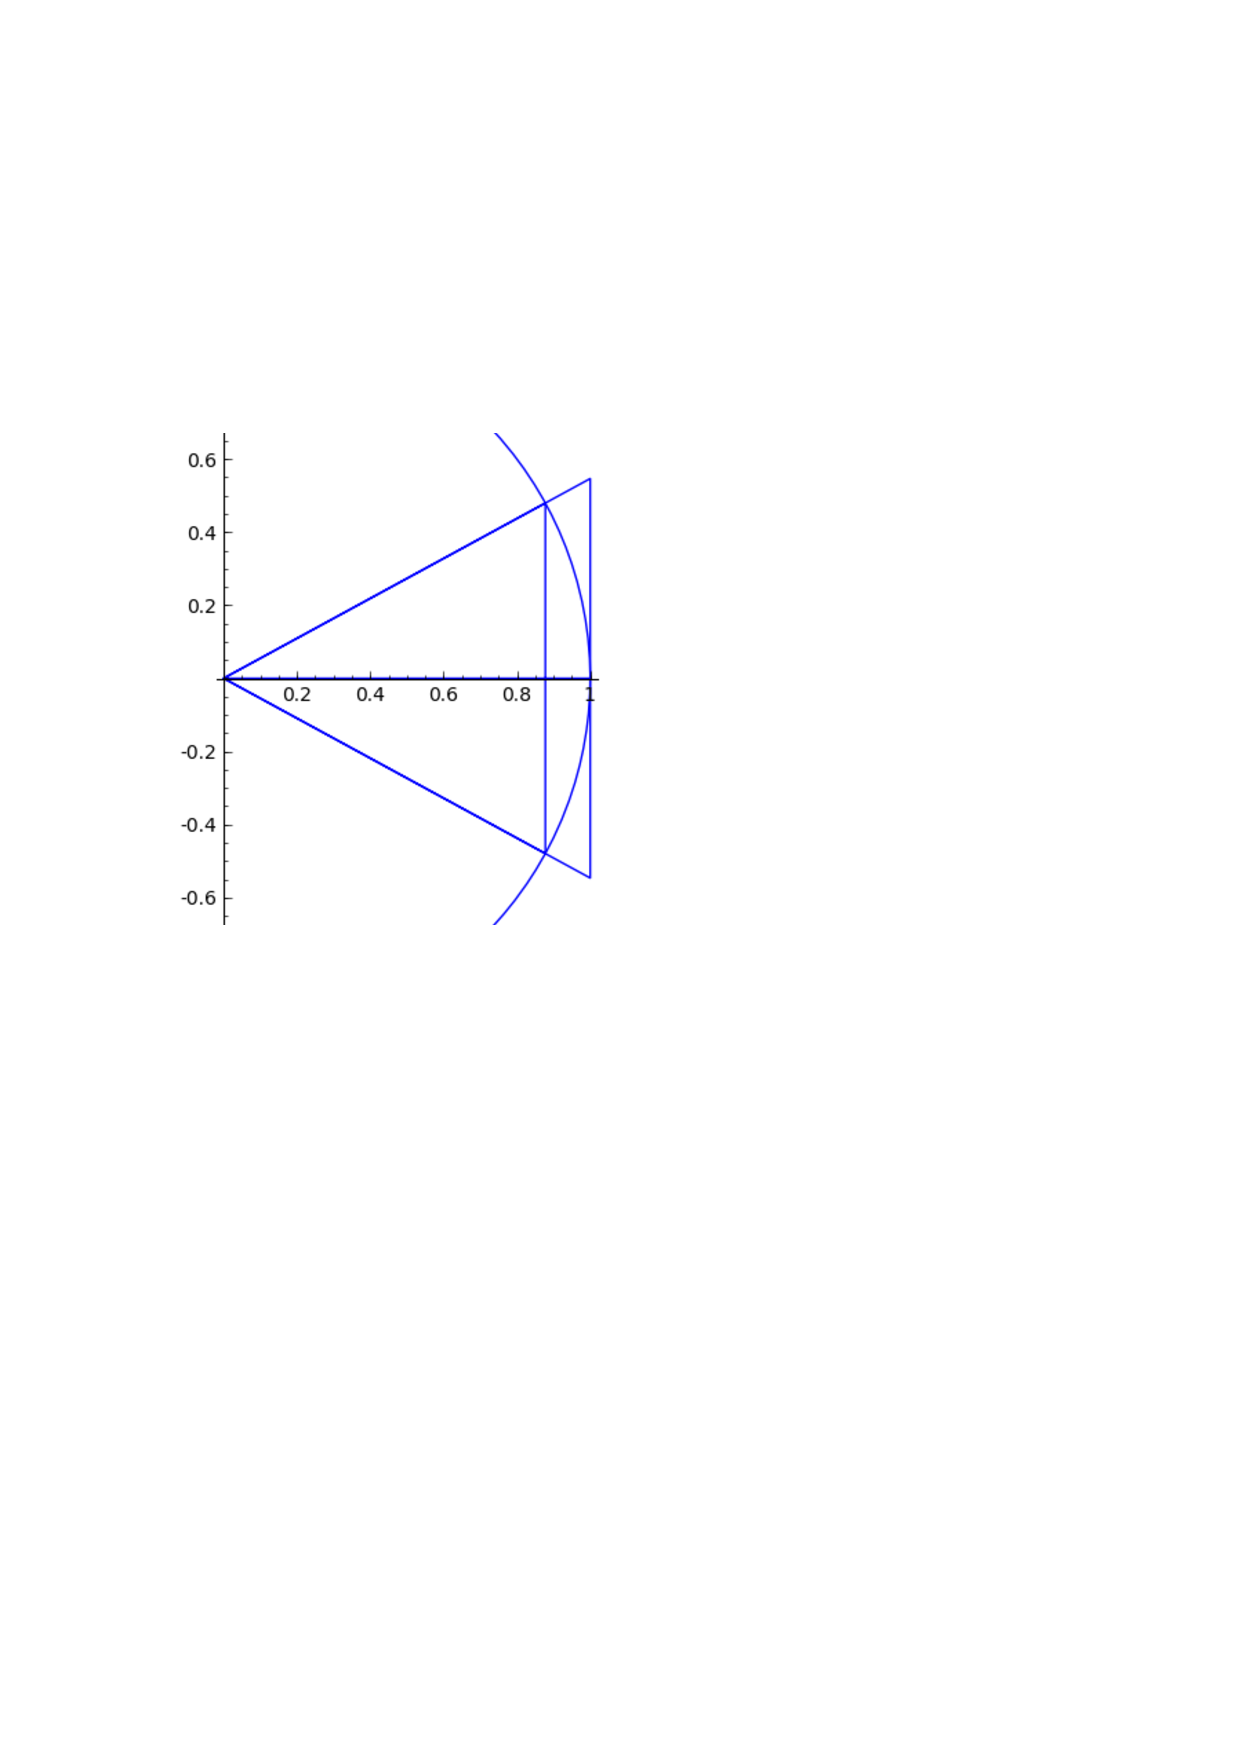
\includegraphics[totalheight=40mm]{imagenes/polincir}
\end{center}
Pero Arqu\'{\i}medes no dispon\'{\i}a de esas funciones trigonom\'etricas, ni de
una calculadora que le diese el valor de 
$\pi$, de forma que lo que hizo fu\'e construir un procedimiento recursivo que
relacionaba los per\'{\i}metros de un pol\'{\i}gono regular inscrito de $n$
lados
y el de $2n$ lados. 

\bigskip \pagebreak[3]
\begin{ejer}
\begin{enumerate}
\item  Utilizar la sucesi\'on $p_n$ para {\itshape calcular} aproximaciones a
$2\pi$.
Como debemos usar un valor aproximado de $\pi$ para poder calcular $p_n$ este
m\'etodo es una
{\itshape tonter\'{\i}a}. Veremos m\'etodos mejores.
\item ?`Por qu\'e es convergente la sucesi\'on $p_n$?  Contestar requiere un
argumento matem\'atico.
\item ?`C\'omo podemos {\itshape ver} en las aproximaciones num\'ericas que la
sucesi\'on es de Cauchy?
\end{enumerate}
\end{ejer}

Sin embargo, es posible, y as\'{\i} lo hizo Arqu\'{\i}medes,  calcular los
per\'{\i}metros de manera recursiva utilizando como valores iniciales los
per\'{\i}metros de los hex\'agonos regulares inscrito y circunscrito a la
circunferencia de radio unidad. Denotemos por $\ell(AB)$ la longitud del
segmento $AB.$

Empezamos con  dos hex\'agonos, que tienen 

\hfil $p_6=6$ , $P_6=6/\cos(\pi/3)=2\sqrt3$

Llamemos 2$\alpha$ al \'angulo que vemos en el origen en la siguiente figura,
desde el eje $OX$ hasta el segundo radio azul, y
supongamos que abarcase uno 
de los lados del pol\'{\i}gono de $2n$ lados \emph{inscrito} en el c\'{\i}rculo
(la cuerda $CD$ que  vemos en la figura).
Llamaremos:
\begin{enumerate}
 \item $S_{2n}:=\ell(CG)$ es la mitad de la longitud del lado del pol\'{\i}gono
regular de $2n$ lados inscrito en la circunferencia.
 
 \item $S_{n}:=\ell(CB)$ es la mitad de la longitud del lado del pol\'{\i}gono
regular de $n$ lados inscrito en la circunferencia.

\item $T_{2n}:=\ell(CF)$ es la mitad de la longitud del lado del pol\'{\i}gono
regular de $2n$ lados circunscrito a la circunferencia.
 
 \item $T_{n}:=\ell(ED)$ es la mitad de la longitud del lado del pol\'{\i}gono
regular de $n$ lados circunscrito a la circunferencia.
 
\end{enumerate}

As\'{\i} que los per\'{\i}metros con $n$ lados son: $p_n=2nS_n$ , $P_n=2nT_n$ .
\begin{center}
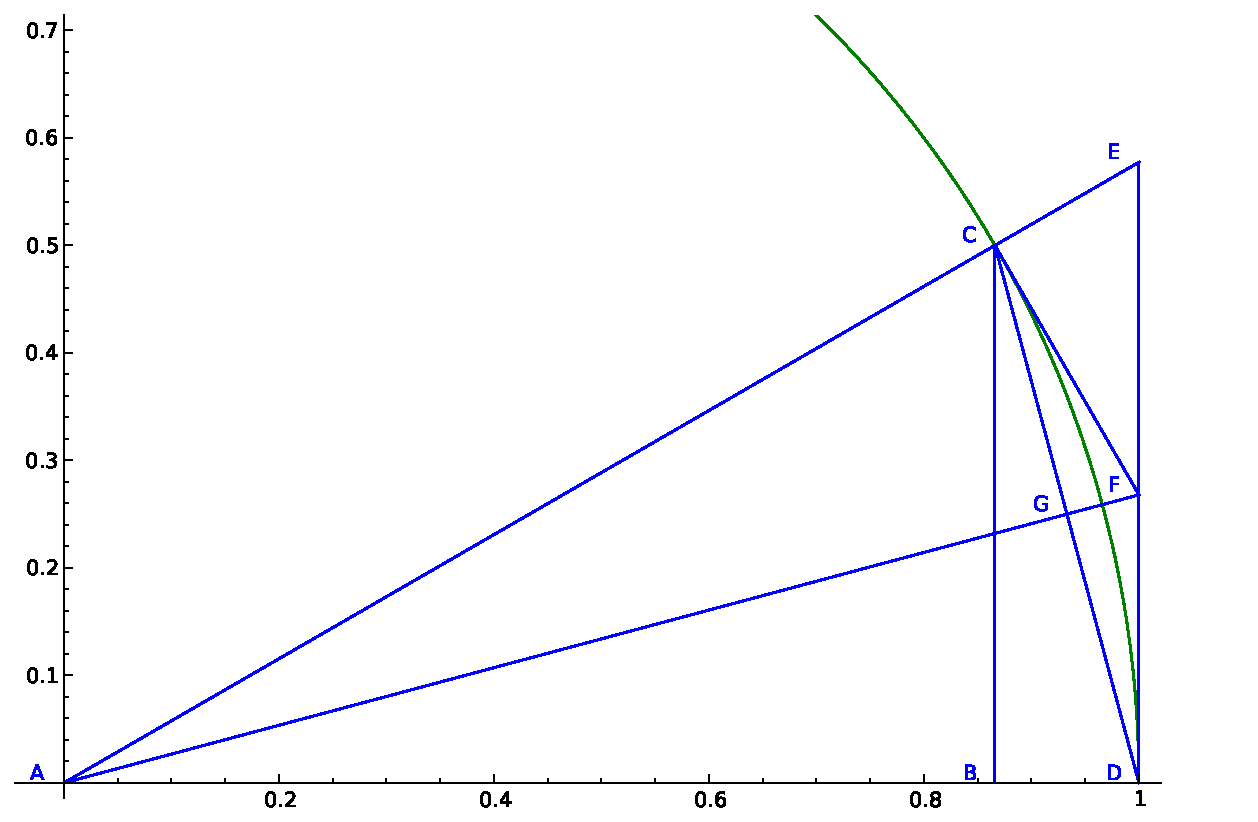
\includegraphics[totalheight=60mm]{imagenes/pi-arqui}
\end{center}

Debe ser claro que:
\begin{enumerate}
\item \label{sem1}Los tri\'angulos $\triangle ABC,\triangle ADE$ y $\triangle
EFC$ son los tres semejantes entre s\'{\i}.
\item \label{sem2} Los tri\'angulos $\triangle ADF, \triangle CGF$ y $\triangle
CBD$ son tambi\'en
semejantes entre s\'{\i}.
\item \label{ig1}Los tri\'angulos $\triangle ACF$ y $\triangle ADF$ son iguales.
\end{enumerate}
Como consecuencia se obtienen las siguientes relaciones:

\begin{enumerate}
 \item (Usando \ref{sem1} y \ref{ig1})
  \[\frac{BC}{DE}=\cos(2\alpha)=\cos(\widehat{AFE})=\frac{CF}{FE},\]
es decir,
 \[\frac{S_n}{T_n}=\frac{T_{2n}}{T_n-T_{2n}},\]
y operando
 \[\frac{T_n}{S_n}=\frac{T_n-T_{2n}}{T_{2n}}=\frac{T_n}{T_{2n}}-1\]
y finalmente
\begin{center}
\fcolorbox{black}{LightYellow}{$T_{2n}=\frac{1}{\frac{1}{T_n}+\frac{1}{S_n}}.$}
\end{center}
 
 \item (Usando \ref{sem2})
 \[\frac{\ell(CB)}{\ell(CD)}=\cos(\alpha)=\frac{\ell(CG)}{\ell(CF)},\]
y, por tanto,
\[\frac{S_n}{2S_{2n}}=\frac{S_{2n}}{T_{2n}},\]
\noindent de donde 
\begin{center}
\fcolorbox{black}{LightYellow}{$S_{2n}=\sqrt{\frac{T_{2n}S_n}{2}}.$}
 \end{center}
\end{enumerate}
Estas f\'ormulas permiten entonces calcular $(S_{2n},T_{2n})$ supuesto que
conocemos $(S_{n},T_{n})$, y partiendo 
de $(S_6,T_6)=(1/2,1/\sqrt{3})$ como caso inicial podemos calcular los
per\'{\i}metros de los pol\'{\i}gonos regulares inscrito y circunscrito con
n\'umero de lados de la forma $6\cdot 2^k$, y as\'{\i} aproximar la longitud de
la circunferencia $2\pi$ como 
\[\lim_{k\to \infty}2(6\cdot 2^k)S_{6\cdot 2^k}=\lim_{k\to \infty}2(6\cdot
2^k)T_{6\cdot 2^k}. \]

\begin{ejer}

Implementa en {\sage} este algoritmo de Arqu\'{\i}medes para aproximar $\pi$,
calculando hasta que la diferencia entre el per\'{\i}metro del pol\'{\i}gono
circunscrito y el del inscrito sea menor que $10^{-n_0}$ para un cierto $n_0$
fijado {\itshape a priori.}
\end{ejer}
%\
%\bigskip
%\

%\href{http://localhost:8080/home/admin/0/}{UNA SOLUCI\'ON}




\subsection{Leonhard Euler (1707-1783)}

Con lo mucho que se hab\'{\i}a aprendido desde Arqu\'{\i}medes, Euler ya
sab\'{\i}a que
$\arctan(x)^{\prime} = 1/(1+x^2)$,
y que para $|x|<1$, podemos ver esa fracci\'on como la suma de una progresi\'on
geom\'etrica de raz\'on $-x^2$ 
y tratar de  ``integrar esa suma infinita t\'ermino a t\'ermino como si fuese un
polinomio'':

\[\frac{1}{1+x^2} = 1-x^2+x^4-x^6+x^8-\cdots\]

\noindent que nos da, integrando t\'ermino a t\'ermino, 

\begin{equation}\label{euler1}
\arctan(x) = x -\dfrac{x^3}{3} +\dfrac{x^5}{5}-\dfrac{x^7}{7}
+\dfrac{x^9}{9} -\cdots
\end{equation}

Como $\tan(\pi/4) = 1$ , eso da una manera de aproximar $\pi/4$ , sumando para
$x=1$, pero muy lenta y, por tanto, muy poco eficiente.

La ingeniosa idea de Euler fue que, en vista de que \quad 
$\tan(a+b) = (\tan(a)+\tan(b))/(1-\tan(a)\tan(b))$,
los \'angulos\\ $a=\arctan(1/2)$, $b=\arctan(1/3)$ suman $\pi/4$, y la suma
(\ref{euler1}) 
para esos valores de $x$, m\'as pr\'oximos a $0$,  converge mucho m\'as
r\'apido.
\
\smallskip
\

\begin{ejer}

Implementa en {\sage}   ambas formas de aproximar $\pi$ (sumando
(\ref{euler1}) para $x=1$ y sumando los valores que se obtienen para $x=a$ y
$x=b$) y compara la eficiencia de los dos m\'etodos.
\end{ejer}
\subsection{Srinivasa Ramanujan (1914)}
Hemos visto un m\'etodo, debido a Euler, para aproximar $\pi$. En este
ejercicio consideramos otro, mucho
m\'as reciente y debido a S. Ramanujan.
\begin{ejer}

\begin{enumerate}
\item Define una funci\'on de  {\sage}  {\tt suma(N)} que devuelve el valor de
la
suma
\[\sum_{n=0}^{n=N}\frac{((2n)!)^3\cdot (42n+5)}{(n!)^6\cdot (16^{(3n+1)})}.\]
\item Comprueba que $1/\text{\tt suma(N)}$ se aproxima a $\pi$ cuando $N$ crece.
\item Intenta estimar, produciendo un programa adecuado, cuantas cifras
correctas de $\pi$ se obtienen cada vez que a\~nadimos~$10$ sumandos m\'as a 
{\tt suma(N)}, es decir, cada vez que incrementamos {\tt N} en $10$ unidades.
\end{enumerate}
\end{ejer}
\subsection{Salamin y Brent (1976)}\label{iterat}

Este algoritmo difiere de los otros que estamos viendo en el hecho de que no se
basa en una serie que converge a $\pi$ sino en un proceso iterativo que produce
una sucesi\'on que converge a $\pi$. Entonces, es similar al algoritmo utilizado
por Arqu\'{\i}medes. 

Se parte de los valores iniciales $a_0=1,\ b_0=\frac{\sqrt{2}}{2}$ y $s_0=1/2$ y
se itera de acuerdo a las f\'ormulas
\begin{equation}\notag
 \begin{aligned}
  a_k&:=\frac{a_{k-1}+b_{k-1}}{2} \\
   b_k&:=\sqrt{a_{k-1}b_{k-1}} \\
   c_k&:=a_k^2-b_k^2 \\
   s_k&:=s_{k-1}-2^kc_k \\
   p_k&:=\frac{2a_k^2}{s_k} \\
 \end{aligned}
\end{equation}
\noindent y $p_k$ es una sucesi\'on con l\'{\i}mite $\pi$. Lo interesante de
este algoritmo es que en cada paso de la iteraci\'on se {\sc duplica} el
n\'umero de cifras correctas de $\pi$ obtenidas, mientras que los algoritmos
basados en series t\'{\i}picamente suman un cierto valor constante, que depende
de la serie,  al  
n\'umero de cifras correctas que ten\'{\i}amos cada vez que a\~nadimos un
sumando m\'as.

Sin embargo, aunque este algoritmo es {\itshape en teor\'{\i}a} muy potente,
cuando se
implementa no es mejor que algoritmos eficientes basados en series debido
simplemente a que el tiempo que tarda el ordenador en  realizar cada
paso de $p_{k-1}$ a $p_k$  crece mucho con $k$. 

\begin{ejer}

Implementa el algoritmo de Salamin y Brent y compara su eficiencia con la del
m\'etodo basado en  la serie de Ramanujan.
\end{ejer}


\subsection{Chudnovsky (199*)}\label{chud}

Otra serie, una variante de la de Ramanujan debida a los hermanos
Chudnovsky,   que permite aproximar   $\pi$ de manera todav\'{\i}a m\'as
eficiente es 

\[S(N):=\sum_{n=0}^{n=N}\frac{(-1)^n\cdot (6n)!)\cdot
(545140134n+13591409)}{(3n!)\cdot (n!)^3\cdot (640320^{3n})},\]

\noindent con la que se obtiene 
\[\pi= \lim_{N\to \infty}\frac{426880*\sqrt{10005}}{S(N)}.\]

Cuando programamos esta f\'ormula no conocemos {\itshape a priori} el n\'umero
de sumandos que necesitamos para obtener una cantidad de d\'{\i}gitos de $\pi$
correctos fijada de antemano. En consecuencia, nos conviene utilizar un bucle
{\tt while} y la \'unica dificultad consiste en formular la condici\'on de
parada adecuada. 


Definimos

\begin{lstlisting}
def F(m):
    A = 545140134
    B = 13591409
    C = 640320
    return
((-1)^m*(factorial(6*m))*(A*m+B))/(factorial(3*m)*(factorial(m)^3)*(C^(3*m)))
 
def pi_chudnovski(ndigits):
    k = 0
    S = 0 
    while 1:
        S += F(k)
        if floor(abs(10^ndigits*F(k))) == 0:
            break
        k += 1
    return (426880*sqrt(10005).n(d${}$igits=ndigits))/S,k
\end{lstlisting}

Estudia con cuidado este programa y, en particular, explica el uso de 
\lstinline|while 1: $\dots$ if $\dots$ :break|. ?`Cu\'al es la justificaci\'on
de la condici\'on de
parada  \lstinline|floor(abs(10^ndigits*F(k))) == 0|?

El programa anterior no es muy eficiente, pero admite muchas mejoras. La primera
consiste en observar que si escribimos 
\[a_n:=\frac{(-1)^n(6*n)!}{(3n)!(n!)^3640320^{3n}},
b_n:=\frac{(-1)^n(6*n)!n}{(3n)!(n!)^3640320^{3n}},\]
\noindent tenemos 
\[\pi=\frac{426880\sqrt{10005}}{B\sum_{n=0}^{\infty}a_n+A\sum_{n=0}^{\infty}
b_n},\]
\noindent pero $b_n=n\cdot a_n$ y  el cociente $a_n/a_{n-1}$ vale 

\[
\frac{(-1)(6n)(6n-2)(6n-3)(6n-4)(6n-5)}{640320^3n^3(3n)(3n-1)(3n-2)}.
\]

Entonces, si ya hemos calculado $a_{n-1}$, es f\'acil, es decir no requiere muchas multiplicaciones, obtener,  a partir de $a_{n-1}$, los valores de $b_{n-1},a_n$ y $b_n$.




 En resumen, podemos calcular cada t\'ermino en la serie en
funci\'on del anterior sin necesidad de repetir una inmensidad de
multiplicaciones que ya se hab\'{\i}an hecho. 

\begin{ejer}

Modifica el programa dado para incluir esta mejora. 
\end{ejer}

Cuando se implementa  este truco, y otros similares,  y se programa en un lenguaje de
programaci\'on compilado, como por ejemplo~$C$, 
este m\'etodo es enormemente eficiente y permite calcular millones de cifras de
$\pi$ en segundos. Como curiosidad puedes
ejecutar las siguientes l\'{\i}neas en una terminal para ver un tal programa en
acci\'on:
\begin{lstlisting}[basicstyle=\color{black},language={C},backgroundcolor=\color{
LightYellow},numbers=left,linewidth=.99\textwidth]
gcc ~/Desktop/SAGE-noteb/bin/gmp-chudnovsky.c -lgmp -lm -O2 -o  ~/Desktop/pi-chudnovsky 
chmod +x ~/Desktop/pi-chudnovsky
~/Desktop/pi-chudnovsky 10000000 1 > ~/Desktop/pi-diez-millones.txt
\end{lstlisting}



?`Por qu\'e es mucho m\'as eficiente un programa escrito en $C$ que el
equivalente en Python?

%\href{http://localhost:8080/home/admin/5/}{HOJA}.


\subsection{Rabinowitz y  Wagon (1995)}


Otra serie que permite calcular d\'{\i}gitos de $\pi$ de forma bastante
eficiente es  


\[\pi=\sum_{n=0}^{\infty}\frac{(n!)^22^{n+1}}{(2n+1)!}.\]

\begin{ejer}

Implementa este c\'alculo en {\sage} , teniendo en cuenta que una
simplificaci\'on 
como la de la secci\'on anterior es posible, y trata de entender cu\'antos
sumandos son necesarios para obtener cada cifra adicional de $\pi$.
\end{ejer}




\subsection{?`Cu\'al es la cifra que ocupa el lugar $1000001$ en $\pi$? (BBP)}

Es cuando poco sorprendente que exista un algoritmo eficiente que permite 
responder
a esa pregunta sin que sea necesario calcular las cifras anteriores. El
c\'alculo se basa en la serie 

\begin{equation}\label{picifras}
\pi=\sum_{k=0}^{k=\infty}\frac{1}{16^k}\Big(\frac{4}{8k+1}-\frac{2}{8k+4}-\frac{
1}
{8k+5}-\frac{4}{8k+6}\Big),
\end{equation}

\noindent y en las siguientes observaciones:
\begin{enumerate}
 \item La parte m\'as costosa del c\'alculo es el de las potencias de $16$.
\'Esto sugiere que puede ser \'util
 tratar de realizar este c\'alculo m\'odulo enteros adecuadamente elegidos y
usando el truco que ya conocemos para calcular r\'apido las potencias. 
 
 \item Si queremos calcular la cifra $n$-\'esima, contando a partir del punto
decimal, debemos multiplicar la expresi\'on decimal de~$\pi$ por $10^n$ y la
cifra que nos interesa es la primera cifra decimal del n\'umero
que obtenemos.
 
Teniendo en cuenta que todos los t\'erminos de la serie tienen un factor de la
forma $1/16^k$,  es claro que multiplicar por potencias de $10$ no es muy
conveniente y debemos usar el sistema de numeraci\'on en base $16$
(hexadecimal). Por tanto, para obtener la $n$-\'esima cifra hexadecimal de $\pi$
debemos multiplicar la serie por $16^n$ y observar la primera cifra despu\'es
del punto.
 
 \item Cuando queremos la cifra $n$-\'esima observamos que en 
 
 
 \begin{equation}\label{picifras2}
 16^n\pi=\sum_{k=0}^{k=\infty}16^{n-k}\Big(\frac{4}{8k+1}-\frac{2}{8k+4}-\frac{
 1}
 {8k+5}-\frac{4}{8k+6}\Big),
 \end{equation}
 
 
 
 
hay dos clases de sumandos: sumandos en los que el exponente de $16$ verifica $n-k\ge 0$ y el resto de los
sumandos.  

Consideremos un sumando como $16^{n-k}/(8k+1)$ con $n-k\ge 0$: como s\'olo  nos
interesa la parte decimal del resultado podemos sustituir esta fracci\'on por 
 $(16^{n-k}\%(8k+1)/(8k+1)$ y obtenemos la misma contribuci\'on al resultado
final. 
 
 Lo importante aqu\'{\i} es que, como ya sabemos, el c\'alculo de potencias
m\'odulo 
 un entero se puede hacer de forma much\'{\i}simo m\'as r\'apida que en los
n\'umeros enteros.
 
 El resto de los sumandos contribuyen cantidades muy peque\~nas a la suma,  y
enseguida podemos dejar de sumarlos porque no afectan al resultado final.
 
 \end{enumerate}
 
%% \newpage
 
 \begin{lstlisting}
def F0(j,m):
    '''Sumandos con m-k no negativo'''
    S =RR(0.0)
    k =0 
    while k <= m:
        r = 8*k+j
        S+=RR(power_mod(16,n-k,r)/r)-floor(RR(power_mod(16,n-k,r)/r))        k += 1
    return RR(S)  
 
def F1(j,m):
    '''Resto de los sumandos'''
    S =RR(0.0)
    k =m+1
    while 1:
        r = 8*k+j
        nS = S+ RR(16^(m-k)/r)
        if S == nS:
            break
        else:
            S = nS
        k += 1
    return RR(S)
    
def S(j,m):
    return RR(F0(j,m)+F1(j,m))
def cifra_pi(n):
    n -= 1
    x = (4*RR(S(1,n))-2*RR(S(4,n))-RR(S(5,n))-RR(S(6,n)))
    return (x-floor(x)).str(base=16)
\end{lstlisting}

\

%%\pagebreak[3]

{\sc Comentarios:}
 
 \begin{enumerate}
  \item Este algoritmo fu\'e descubierto por Bayley, Borwein y Plouffe en 1997.
Puedes ver el art\'{\i}culo original en
\href{http://150.244.21.37/PDFs/APROX/digits-BBP.pdf}{este enlace.}
  
  \item Estudia cuidadosamente este programa, fij\'andote en particular en 
  \begin{enumerate}
  \item el uso que se hace de los n\'umeros reales de precisi\'on doble ({\tt RR}). 
 % % \item las l\'{\i}neas que terminan en {\tt\%1.0}. % %
  \item la forma de transformar el resultado a hexadecimal en la \'ultima
l\'inea. 
  \end{enumerate}
\item Antes del descubrimiento de esta clase de algoritmos se pensaba que para
calcular la $n$-\'esima cifra de $\pi$ hab\'{\i}a que efectuar todo el
c\'alculo, por ejemplo sumando una serie,  con m\'as de $n$ d\'{\i}gitos de
precisi\'on y, por supuesto, durante el proceso se calculaban todas las cifras
anteriores. 

En cambio, en este algoritmo se usan n\'umeros reales de precisi\'on doble
independientemente de lo grande que sea $n$. La~cantidad de memoria RAM que usa
el programa es 
muy reducida porque se reutiliza todo el tiempo la misma memoria.

\item Es posible obtener un rendimiento mucho mayor del algoritmo
program\'andolo en C, o usando \hyperref[cython]{Cython.} 
%%%%%%ERRORES EN LA VERSION ACTUAL EN CYTHON 07-06-2013%%%%%%%%%%

\end{enumerate}
 
\
 
 \bigskip
 
 \
 
 
\begin{ejer}

\begin{enumerate}
 \item Hay otras constantes de las que podemos calcular la cifra $n$-\'esima sin
calcular las anteriores. Por ejemplo, se puede usar la serie
 \[\log(2)=\sum_{k=1}^{\infty} \frac{1}{k2^k},\]
 para calcular cifras del logaritmo neperiano de $2$. Modifica el programa
anterior para adaptarlo a este caso.
 
 ?`Cu\'al podr\'{\i}a ser la forma general de series a las que se les puede
aplicar este m\'etodo?
 
 \item Intenta adaptar este programa para calcular, de manera eficiente (i.e.
evitando en lo posible repetir c\'alculos que ya se han hecho),  
 $N$ cifras consecutivas de $\pi$ empezando en la que ocupa el lugar $n_0$. 
 \end{enumerate}
\end{ejer}


%\href{http://localhost:8080/home/admin/4/}{HOJA}.


\subsection{Aproximaciones racionales de $\pi$}

Debemos saber que \href{http://150.244.21.37/PDFs/APROX/pi-irracional.pdf}{$\pi$ no es un
n\'umero racional}, es decir, su
expresi\'on como un decimal no es peri\'odica. Sin embargo, hay fracciones que
aproximan bastante bien el valor de $\pi$.

Cuando calculamos cualquier valor aproximado de  $\pi$, como un decimal con un
cierto n\'umero de cifras despu\'es del punto,  estamos calculando un n\'umero
racional pr\'oximo a $\pi$, pero se trata de n\'umeros racionales con
denominador
una potencia de~$10$. Tambi\'en podemos usar series de sumandos racionales que
aproximan $\pi$ lo que nos da, al efectuar la suma finita, n\'umeros racionales
pr\'oximos a $\pi$, y ahora el denominador  no ser\'a, en general,  una potencia
de diez.

En este ejercicio buscamos la mejor aproximaci\'on racional de $\pi$ con un
n\'umero, acotado a priori, de cifras en el denominador. En estas condiciones,
podemos intentar un enfoque de \hyperref[bruta]{\itshape fuerza bruta} ya que,
fijado un entero
positivo $k$,  hay un n\'umero finito de fracciones $a/b$ tales que, por
ejemplo,  $3{.}14<a/b<3{.}15$ y $0<b<10^k$ (?`por qu\'e?). 

Algunas de esas aproximaciones son muy buenas, en el sentido de que teniendo un
denominador no muy grande nos dan un n\'umero inesperadamente grande de cifras
correctas de $\pi$.

%  Debemos saber que $\pi$ no es un n\'umero racional, es decir, su
% expresi\'on como un decimal no es peri\'odica. Sin embargo, hay fracciones que
% aproximan bastante bien el valor de $\pi.$
 \begin{ejer}
 
 \begin{enumerate}
 \item Define una funci\'on de {\sage}  que encuentre, y devuelva,  la
fracci\'on,
con denominador de como m\'aximo  $k$ cifras (en base~$10$), que mejor aproxime
a $\pi.$ 
 
 \footnotesize
 {\sc No se permite} usar el m\'etodo \lstinline|exact_rational()| de {\sage} ,
que
m\'as o menos puede hacer lo que se pide en el ejercicio. {\sc S\'{\i} se
puede} 
usar el valor de $\pi$ que tiene internamente {\sage}.
 
 ?`Cu\'antos bucles tendr\'a tu funci\'on?
 \normalsize
 
 \item Jugando con los rangos de los bucles, pero sin usar expl\'{\i}citamente
los resultados mencionados m\'as abajo,  trata de conseguir un programa lo m\'as
eficiente posible. 
 
 \footnotesize
 \bigskip
 {\sc Algunos resultados:}
 
 \begin{enumerate}
  \item Con denominador de $3$ cifras, como m\'aximo, se obtiene la fracci\'on
$355/113$, con un error del orden de $3\times 10^{-7}$. 

\item Con denominador de $4$ cifras, como m\'aximo, se obtiene la misma
fracci\'on $355/113$ como la mejor aproximaci\'on.  En mi m\'aquina tarda   $10$
segundos. 

\item Con denominador de $5$ cifras, como m\'aximo, se obtiene la fracci\'on
$312689/99532$, con un error del orden de $3\times 10^{-11}$. En mi m\'aquina 
tarda   $100$ segundos. 
 \end{enumerate}

\end{enumerate}
\end{ejer}

%\href{http://localhost:8080/home/admin/?/}{HOJA}.


\section{Fracciones Continuas}
\def\floor#1.{\lfloor #1\rfloor}

\noindent\textbf{Las fracciones continuas aparecen al dividir. } Consideramos la
fracci\'on $\frac{55}{43}$. Al aplicar el algoritmo de Euclides para calcular el
m\'aximo com\'un divisor de 55 y 43, obtenemos como pasos intermedios las
expresiones
$$
\begin{array}{rcl}
55&=&1\cdot 43+12,\\
43&=&3\cdot 12+7,\\
12&=&1\cdot 7+5,\\
7&=&1\cdot 5+2,\\
5&=&2\cdot 2+1,\\
2&=&2\cdot 1+0.
\end{array}
$$
Los n\'umeros 1, 3, 1, 1, 2, 2 son los cocientes parciales del algoritmo. 
Utilizando esta informaci\'on podemos escribir la fracci\'on $\frac{55}{43}$ de
una forma curiosa:
$$
\begin{array}{l}
\frac{55}{43}=1+\frac{12}{43}=1+\frac1{\frac{43}{12}}=1+\frac1{3+\frac7{12}}
=1+\frac1{3+\frac1{1+\frac57}}=1+\frac1{3+\frac1{1+\frac1{2+\frac25}}}
=1+\frac1{3+\frac1{1+\frac1{1+\frac1{2+\frac12}}}}.
\end{array}
$$
La expresi\'on de m\'as a la derecha de esta cadena de igualdades es lo que se
conoce como una fracci\'on continua (simple) finita. Para describirla de una
forma m\'as compacta, utilizaremos en lo que sigue cualquiera de las dos
notaciones siguientes:
$$
1+\frac1{3+\frac1{1+\frac1{1+\frac1{2+\frac12}}}}=1+\frac1{3+}\frac1{1+}\frac1{
1+}\frac1{2+}\frac12=[1;3,1,1,2,2].
$$

No hay nada de especial en los n\'umeros 55 y 43. Podemos seguir el mismo
procedimiento con dos enteros cualesquiera, $a$, $b$ con $a\ne0$ para escribir
$b/a$ como una fracci\'on continua finita.

\noindent\emph{Observaci\'on. }
La representaci\'on de un racional como fracci\'on continua finita no es
\'unica, ya que, si $a_n\ge2$, tenemos que
$$
[a_0;a_1,\dots,a_n]=[a_0;a_1,\dots, a_n-1,1],
$$
mientras que si $a_n=1$ podemos escribir
$$
[a_0;a_1,\dots,a_{n-1},1]=[a_0;a_1,\dots, a_{n-1}+1].
$$
Sin embargo, estas son las \'unicas ambig\"uedades posibles y, si hacemos la
hip\'otesis de que el \'ultimo cociente parcial sea siempre mayor que 1,
$a_n>1$, entonces la representaci\'on de un n\'umero racional como fracci\'on
continua es \'unica.


\noindent\textbf{Las fracciones continuas aparecen al resolver ecuaciones. }
Consideramos la ecuaci\'on $x^2-x-1=0$. Su \'unica soluci\'on positiva es la
raz\'on \'aurea, $\Phi=\frac{1+\sqrt{5}}2$. Podemos reescribir $\Phi^2-\Phi-1=0$
como $\Phi=1+\frac1\Phi$. Sustituyendo la $\Phi$ del denominador por
$\Phi=1+\frac1\Phi$ obtenemos
$$
\Phi=1+\frac1{1+\frac1\Phi}.
$$
Repitiendo este proceso de sustituci\'on \lq\lq hasta el infinito\rq\rq, podemos
escribir
$$
\text{\lq\lq}\Phi=1+\frac1{1+\displaystyle\frac1{1+\displaystyle\frac1{
1+\displaystyle\frac1{1+\ddots}}}}.\text{\rq\rq}
$$
El lado derecho de esta expresi\'on es un ejemplo de una fracci\'on continua
infinita. ?`Por qu\'e hemos puesto la igualdad entre comillas? Porque tenemos
que dar sentido al lado derecho de la expresi\'on, a la fracci\'on continua
infinita. 


\noindent\textbf{Fracciones continuas infinitas. Convergentes. } 
Sea $a_0$ un entero arbitrario (positivo, negativo o cero),  y
$\{a_j\}_{j=1}^\infty$, una sucesi\'on de enteros positivos. 
Llamamos $n$-\'esimo convergente de la fracci\'on continua infinita (simple)
$[a_0;a_1,a_2,\dots]$ a la fracci\'on continua finita $c_n=[a_0;a_1,\dots,a_n]$.
N\'otese que $c_n$ est\'a bien definido, y que es un n\'umero racional. Si el
l\'{\i}mite $\lim_{n\to\infty}c_n$ existe, decimos que la fracci\'on continua
infinita $[a_0;a_1,a_2,\dots]$ converge, y denotamos
$[a_0;a_1,a_2,\dots]=\lim_{n\to\infty}c_n$.




Un sencillo argumento de inducci\'on permite demostrar que los convergentes
$c_n=[a_0;a_1,\dots,a_n]$ verifican
$$
c_n=\frac{p_n}{q_n},
$$
donde las sucesiones $\{p_n\}$ y $\{q_n\}$ vienen dadas por las relaciones de
recurrencia de Wallis-Euler, 
$$
\begin{array}{llll}
p_0=a_0,\qquad& p_1=a_0a_1+1,\qquad &p_n=a_np_{n-1}+p_{n-2},\quad &n\ge 2\\
q_0=1,\qquad& q_1=a_1,\qquad &q_n=a_nq_{n-1}+q_{n-2},\quad &n\ge 2.
\end{array}
$$
No es dif\'{\i}cil demostrar a partir de aqu\'{\i} que
$$
\begin{array}{l}
p_nq_{n-1}-q_np_{n-1}=(-1)^{n-1},\\
p_nq_{n-2}-q_np_{n-2}=(-1)^{n}a_n,
\end{array}
 \qquad n=1,2,\dots
$$
Como consecuencia inmediata se obtiene que $p_n$ y $q_n$ son coprimos. Adem\'as,
aplicando sucesivas veces estas identidades se obtiene que
$$
c_n-c_{n-1}=\frac{(-1)^{n-1}}{q_nq_{n-1}},\quad n\ge 1,\qquad
c_{n}-c_{n-2}=\frac{(-1)^n a_n}{q_nq_{n-2}},\quad n\ge2.
$$
Por otra parte, $q_n<q_{n+1}$ para todo $n\ge0$, y adem\'as
$\lim_{n\to\infty}q_n=\infty$, por lo que concluimos que las fracciones
continuas infinitas (simples) siempre convergen a un cierto
$\alpha=\lim_{n\to\infty}c_n$, y que los convergentes satisfacen
$$
c_0<c_2<c_4<\cdots<c_{2_n}<\cdots<\alpha<\cdots<c_{2n-1}<\cdots<c_5<c_3<c_1.
$$
Se tiene adem\'as la estimaci\'on
$$
\left|\alpha-c_n\right|<\frac1{q_nq_{n+1}}<\frac1{q_{n}^2},
$$
v\'alida para todos los valores de $n$, lo que implica que $\alpha$ no puede ser
racional.
As\'{\i} pues, una fracci\'on continua (simple) es racional si y s\'olo si es
finita.

\noindent\emph{Ejemplo. } En particular, la fracci\'on continua
$\Phi:=[1;1,1,1,\dots]$ converge. ?`A qu\'e? N\'otese que
$$
\Phi=1+\frac1{1+\displaystyle\frac1{1+\displaystyle\frac1{1+\displaystyle\frac1{
1+\ddots}}}}=1+\frac1\Phi\qquad\Rightarrow \Phi=1+\frac1\Phi.
$$
Tambi\'en podemos obtener esta f\'ormula a partir de los convergentes. En
efecto, el $n$-\'esimo convergente de $\Phi$ es 
$$
c_n=1+\frac1{1+\displaystyle\frac1{1+\displaystyle\frac\ddots{
1+\displaystyle\frac1{1+1}}}}=1+\frac1{c_{n-1}}.
$$
Por lo tanto, si denotamos por $\Phi$ al $\lim_{n\to\infty}c_n$, que sabemos que
existe, tomando $n\to\infty$ en ambos miembros de $c_n=1+\frac{1}{c_{n-1}}$,
obtenemos que $\Phi=1+\frac1\Phi$, igual que antes. Concluimos que $\Phi$ es la
\'unica soluci\'on positiva de $x^2-x-1=0$, es decir,
$$
\Phi=\frac{1+\sqrt{5}}2.
$$ 


\noindent\textbf{Algoritmo can\'onico para obtener la fracci\'on continua de un
n\'umero irracional. } ?`C\'omo construir la expansi\'on en fracciones continuas
de un n\'umero real? Ya sabemos c\'omo hacerlo para n\'umeros racionales; el
mismo m\'etodo, interpretado adecuadamente, funcionar\'a para irracionales, de
manera que vamos a revisarlo. 

Consideramos el n\'umero $\frac{157}{68}=[2;3,4,5]$. Veamos c\'omo se obtiene su
expansi\'on en fracciones continuas. En primer lugar escribimos
$\xi_0:=\frac{157}{68}$ como
$$
\xi_0=2+\frac1{\xi_1}, \qquad \text{donde }\xi_1=\frac{68}{21}>1.
$$
En particular, 
$$
a_0=2=\floor \xi_0.,
$$
donde, para cada n\'umero real $x$, $\floor x.$ denota al mayor entero menor o
igual que $x$. Seguidamente, escribimos $\frac{68}{21}$ como
$$
\xi_1=3+\frac1{\xi_2}, \qquad \text{donde }\xi_2=\frac{21}{5}>1.
$$
En particular,
$$
a_1=3=\floor \xi_1.,
$$
En tercer lugar, escribimos
$$
\xi_2=\frac{21}5=4+\frac1{\xi_3}, \qquad \text{donde }\xi_3=5>1.
$$
En particular,
$$
a_2=4=\floor \xi_2.,
$$
Finalmente, $a_3=\floor \xi_3.=\xi_3$ no se puede descomponer m\'as, de manera
que \emph{paramos} aqu\'{\i}. Por consiguiente,
$$
\frac{157}{68}=\xi_0=2+\displaystyle\frac1{\xi_1}=2+\frac1{3+\displaystyle\frac1
{\xi_2}}=2+\frac1{3+\displaystyle\frac1{4+\displaystyle\frac1{\xi_3}}}
=2+\displaystyle\frac1{3+\displaystyle\frac1{4+\displaystyle\frac1{5}}}
$$
Acabamos de encontrar la fracci\'on continua can\'onica (simple) de $157/68$.
N\'otese que acabamos con el n\'umero 5, que es mayor que 1; este ser\'a siempre
el caso cuando apliquemos el procedimiento a un n\'umero racional no entero. 

Podemos seguir exactamente el mismo procedimiento para los n\'umeros
irracionales:

Sea $\xi$ un n\'umero irracional. Hacemos $\xi_0=\xi$ y definimos
$a_0:=\floor\xi_0.\in\mathbb{Z}$. Entonces, $0<\xi_0-a_0<1$, de forma que
podemos escribir
$$
\xi_0=a_0+\frac1{\xi_1}, \qquad \text{donde }\xi_1:=\frac1{\xi_0-a_0}>1.
$$
N\'otese que $\xi_1$ es irracional. En segundo lugar, definimos
$a_1:=\floor\xi_1.\in\mathbb{N}$. Entonces $0<\xi_1-a_1<1$, de forma que podemos
escribir
$$
\xi_1=a_1+\frac1{\xi_2}, \qquad \text{donde }\xi_2:=\frac1{\xi_1-a_1}>1.
$$
N\'otese que $\xi_2$ es irracional. En tercer lugar, definimos
$a_2:=\floor\xi_1.\in\mathbb{N}$. Entonces $0<\xi_2-a_2<1$, de forma que podemos
escribir
$$
\xi_2=a_2+\frac1{\xi_3}, \qquad \text{donde }\xi_3:=\frac1{\xi_2-a_2}>1.
$$
N\'otese que $\xi_3$ es irracional. Podemos continuar este procedimiento \lq\lq
hasta el infinito\rq\rq, creando una sucesi\'on de n\'umeros reales
$\{\xi_n\}_{n=0}^\infty$ de n\'umeros reales con $\xi_n>0$ para $n\ge1$ llamada
la sucesi\'on de cocientes completos de $\xi$, y una sucesi\'on
$\{a_n\}_{n=0}^\infty$ de enteros con $a_n>0$ para $n\ge1$ llamada la sucesi\'on
de cocientes parciales de $\xi$, tales que
$$
\xi=a_n+\frac1{\xi_{n+1}},\qquad n=0,1,2,3,\dots
$$
Por consiguiente, 
$$
\xi=\xi_0=a_0+\frac1{\xi_1}=\xi_0=a_0+\frac1{a_1+\displaystyle\frac1{\xi_2}}
=\cdots=\text{\lq\lq}=\text{\rq\rq}
a_0+\frac1{a_1+\displaystyle\frac1{a_2+\displaystyle\frac1{
a_3+\displaystyle\frac1{a_4+\ddots}}}}.
$$
No hemos demostrado que $\xi$ sea igual a la fracci\'on continua infinita de la
derecha (de ah\'{\i} las comillas), pero esta igualdad es cierta. 

\

\begin{ejer}

\begin{enumerate}
 \item Escribir un c\'odigo  que, tomando un \mbox{$r > 1$} y un n\'umero
 dado $k$ de pasos, halle los
$[a_0, \dots , a_k ]$ de la fracci\'on
 continua de~$r$.
 
\item Para el caso de un racional $r = n/m > 1$, hacer una variante del c\'odigo
anterior
 que tome los enteros $n$, $m$ como datos y devuelva la lista completa
 $[a_0, \dots , a_k ]$, hasta el fin del desarrollo.

 \item Escribir otra funci\'on  que tome los $[a_0, \dots , a_k ]$ y produzca
las fracciones (convergentes) $c_n=p_n/q_n$, $n=0,...,k$.

\item Escribir una funci\'on  que tome un \mbox{$r > 1$} y una tolerancia
\texttt{tol}, y devuelva una fracci\'on que aproxime $r$ con un error menor  que
\texttt{tol}.

\item Comprueba que las convergentes $c_k$ tienen la siguiente propiedad: el
error de la aproximaci\'on  $c_k$ es menor que el error de cualquier
aproximaci\'on
 con un denominador menor que el denominador de $q_k$. Efect\'ua
 la comprobaci\'on con al menos un n\'umero algebraico
y otro trascendente, para al menos las cuatro primeras aproximaciones~$c_k$.

\end{enumerate}
\end{ejer}


\section{Fracciones continuas periódicas. Números irracionales cuadráticos}
%Quadratic irrationals and periodic continued fractions
Sabemos que, entre los números reales, solo los racionales tienen un desarrollo decimal periódico. Podemos preguntarnos qué hay sobre este asunto en los desarrollos en fracción continua: ¿qué reales tienen fracciones continuas periódicas?

Hemos visto ya algún ejemplo, la razón áurea con desarrollo
$$
\Phi=\frac{1+\sqrt5}2=[1;1,1,1,1,....]
$$
que denotaremos como $[\,\overline 1\,]$ para indicar que el $1$ se repite.

Si tomamos la raíz cuadrada de $8$ se llega a $\sqrt8=[2;1,4,1,4,...]=[2;\overline{1,4}]$, donde tenemos que se repite indefinidamente el bloque $1,4$. En efecto, $\lfloor\sqrt8\rfloor=2$ de manera que:
\begin{align*}
\sqrt8=\destaca2+(\sqrt8-2) \text{ con }\sqrt8-2<1\\
\frac1{\sqrt8-2}=\frac{\sqrt8+2}{8-4}=\frac{\sqrt8+2}{4}
&\text{ donde } 1<\tfrac{\sqrt8+2}{4}<2\\
&\text{ y así }\frac{\sqrt8+2}{4}=1+\left(\tfrac{\sqrt8+2}{4}-1\right)=
\destaca1+\frac{\sqrt8-2}{4}
\text{ con }\tfrac{\sqrt8-2}{4}<1\\
\frac1{\frac{\sqrt8-2}4}=\frac{4(\sqrt8+2)}{8-4}=\sqrt8+2=\destaca4+(\sqrt8-2)
&\text{ con }\sqrt8-2<1\,.
\end{align*}
Y hemos llegado a un valor ya antes visitado en el algoritmo: $\frac1{\sqrt8-2}=\dots$

Antes de ver cómo recuperar $\sqrt8$ a partir de esta fracción continua, veamos otro ejemplo, esta vez con periodo puro. Desarrollemos nuestro algoritmo para $\sqrt7+2$:
\begin{align*}
\sqrt7+2&=\destaca4 +(\sqrt7-2)=\destaca4+\frac1{\frac 1{\sqrt7-2}}\\
\frac1{\sqrt7-2}&=\frac{\sqrt7+2}{3}=\destaca1+\frac{\sqrt7-1}{3}=\destaca1+
\frac1{\frac3{\sqrt7-1}}\\
\frac3{\sqrt7-1}&=\frac{3(\sqrt7+1)}{6}=\frac{\sqrt7+1}{2}=\destaca1+
\frac{\sqrt7-1}{2}=\destaca1+\frac1{\frac2{\sqrt7-1}}\\
\frac2{\sqrt7-1}&=\frac{2(\sqrt7+1)}{6}=\frac{\sqrt7+1}{3}=
\destaca1+\frac{\sqrt7-2}{3}=\destaca1+\frac1{\frac3{\sqrt7-2}}\\
\frac3{\sqrt7-2}&=\frac{3(\sqrt7+2)}{3}=\sqrt7+2\,\, \text{(igual que empezamos)}
\end{align*}
y así: $\sqrt7+2=[\,\overline{4,1,1,1}\,]$.

Podemos recuperar este último valor a partir de la expresión $[\,\overline{4,1,1,1}\,]$. Basta resolver la siguiente ecuación:
\begin{equation}
x=[4,1,1,1,x]\,.\label{ec-1}
\end{equation}
Desarrollando el miembro derecho se obtiene
$$
[4,1,1,1,x]=\destaca4+\frac1{\destaca1+\frac{1}{\destaca1+\frac{1}{\destaca1+\frac1x}}}
=
\destaca4+\frac1{\destaca1+\frac{1}{\destaca1+\frac{x}{x+1}}}
=
\destaca4+\frac1{\destaca1+\frac{x+1}{2x+1}}
=
\destaca4+\frac{2x+1}{3x+2}=\frac{14x+9}{3x+2}\,.
$$
La ecuación \eqref{ec-1} es por tanto una ecuación cuadrática:
$$ x= \frac{14x+9}{3x+2} \,\,\longleftrightarrow\,\,3x^2-12x-9=0$$
y su raíz positiva, $\frac{12+\sqrt{144+108}}6=2+\sqrt7$, es el número buscado.

Con una pequeña variante también se puede recuperar el irracional correspondiente a un desarrollo periódico no puro, como $[2;\overline{1,4}]$. Basta observar que, si $x=[\,\overline{1,4}\,]$, entonces $[2;\overline{1,4}]=[2;x]=2+\frac1x$. Si desarrollamos $x=[1;4,x]$ llegamos a $x=\frac{5x+1}{4x+1}$, de donde a la ecuación cuadrática $4x^2-4x-1=0$. La raíz positiva es $\frac{\sqrt2+1}2$, y 
$$
2+\frac2{1+\sqrt2}=\frac{4+2\sqrt2}{1+\sqrt2}=
(2\sqrt2+4)(\sqrt2-1)=2\sqrt2=\sqrt8\,.
$$

Acabamos de ver cómo una ecuación del tipo:
$$
x=[\,\overline{a_0,a_1,\dots,a_m}\,]=[a_0;a_1,\dots,a_m,x]
$$
nos ha llevado a una ecuación cuadrática, de coeficientes enteros si los $a_i$ son enteros. Si los $a_i$ son positivos, la solución positiva de esta ecuación cuadrática es el irracional con desarrollo en fracción continua periódico $[\,\overline{a_0,a_1,\dots,a_m}\,]$.

El caso periódico más general no es muy distinto, y podemos calcular el irracional con desarrollo 
$$
[a_0;a_1,\dots,a_\ell,\overline{b_0,b_1,\dots,b_m}\,]
$$
a partir del irracional raíz de la ecuación cuadrática
$$x=[b_0,b_1,\dots,b_m,x]\,.$$

Aunque son solo un par de ejemplos, este es un resultado general demostrado por Lagrange (1736--1813). Antes de enunciarlo, algo de notación. Definimos:
\begin{align*}
\mathbb Z[\sqrt d]&:=\big\{a+b\sqrt d: a,b\in\mathbb Z\big\}\\
\mathbb Q[\sqrt d]&:=\big\{a+b\sqrt d: a,b\in\mathbb Q\big\}
\end{align*}
Dado $\xi=a+b\sqrt d$ en $\mathbb Z[\sqrt d]$ o $\mathbb Q[\sqrt d]$, se define su conjugado como $\overline\xi:=a-b\sqrt d$. Con las operaciones obvias, $\mathbb Z[\sqrt d]$ es un anillo conmutativo, y $\mathbb Q[\sqrt d]$ un cuerpo. Además, la conjugación preserva las propiedades algebraicas: si $\alpha,\beta\in\mathbb Q[\sqrt d]$, entonces
$$
\overline{\alpha\pm\beta}=\overline\alpha\pm\overline\beta,\quad
\overline{\alpha\cdot\beta}=\overline\alpha\cdot\overline\beta\,.
$$

Obsérvese que si $d$ es un entero positivo que no es un cuadrado ($\sqrt d\notin\mathbb Z$), y $b\neq0$, $a+b\sqrt d$ es un irracional. Estos irracionales se dicen cuadráticos pues se pueden poner como solución de una ecuación cuadrática con coeficientes enteros:
\begin{align*}
\xi=r+s\sqrt d\in\mathbb Q[\sqrt d] &
\text{ es solución de: } x^2-2r\,x+(r^2-s^2d)=0
\end{align*}
Si multiplicamos por el mínimo común múltiplo de los denominadores de $2r$ y $r^2-s^2d$, se tiene un polinomio cuadrático con coeficientes enteros.

Ahora ya podemos enunciar el resultado de Lagrange:

\begin{Tma}[Lagrange] Una fracción continua simple infinita es un irracional cuadrático si y solo si es periódica.
\end{Tma}

Entre los irracionales cuadráticos los hay con fracción continua periódica pura, ¿quiénes son?

\begin{Tma}[Galois]
	Un irracional cuadrático $\xi$ es puramente periódico si y solo si 
	$$\xi>1\quad\text{ y }\quad -1<\overline\xi<0\,.$$
\end{Tma}

Un caso especialmente llamativo es el de las raíces cuadradas de los enteros (no cuadrados). 
%Estas fueron estudiadas por Adrien-Marie Legendre (1752--1833)

\begin{Tma}\label{Tma-Raizd} %[Legendre]
	Sea $d$ un entero positivo que no es un cuadrado. La fracción continua para $\sqrt d$ es de la forma
	$$
	[a_0;\overline{a_1,\dots,a_{n-1},a_n}\,]
	$$
	con $a_n=2a_0$ y $a_k\le a_0$ para $1\le k< n$.
	
	Además, si $m\ge 1$ y $x=p_{mn-1}$ e $y=q_{mn-1}$ son el numerador y el denominador de la $(mn-1)$-ésima convergente de $\sqrt d$, entonces:
	$$
	x^2-dy^2=\pm 1\,.
	$$
\end{Tma}

\noindent{\sc Observación:} Es un cálculo directo el comprobar que si $x_1, y_1$ son tales que $x_1^2-dy_1^2=-1$, al tomar $x, y$ tales que $x+y\sqrt d=(x_1+y_1\sqrt d)^2$, se tiene que $x^2+dy^2=1$.

Una aplicación directa de este resultado la encontramos en la resolución de las llamadas ecuaciones de Pell.

\subsection{Ecuaciones de Pell}

Una ecuación de Pell es una ecuación diofántica de la forma:
\begin{equation}
x^2-dy^2=1\label{ec-Pell}
\end{equation}
donde $d$ es un entero, y para la que se buscan soluciones enteras positivas. Siempre se tiene la solución trivial $x=1$, $y=0$. Si $d$ es un cuadrado, no existen soluciones enteras no triviales a la ecuación de Pell. Si $d$ no es un cuadrado, existen infinitas soluciones.

Obsérvese que, si $y\neq0$, podemos reescribir la ecuación como
$$
\frac{x^2}{y^2}-d=\frac1{y^2}
$$
y así, $\frac xy$ se acerca a $\sqrt d$. Del Teorema~\ref{Tma-Raizd} se deduce el siguiente algoritmo para encontrar una solución a la ecuación de Pell~\eqref{ec-Pell}.

\begin{quotation}
	\fbox{\begin{minipage}{.8\textwidth}
			\centerline{\bf Resolviendo $\mathbf{x^2-dy^2=1}$}
			\begin{enumerate}
				\item Calcular $a_0=\lfloor\sqrt d\rfloor$.
				\item Calcular la fracción continua $[a_0;a_1,a_2,\dots]$ para $\sqrt d$. Parar cuando $a_n=2a_0$.
				\item Sea $x_1=p_{n-1}$ e $y_1=q_{n-1}$ (el numerador y el denominador de la convergente $n-1$).
				\item Si $x_1^2-dy_1^2=1$, tomar $x=x_1$ e $y=y_1$ y parar.
				\item Si $x_1^2-dy_1^2=-1$, calcular $x+y\sqrt d=(x_1+y_1\sqrt d)^2$. Entonces $x^2-dy^2=1$, y parar.
			\end{enumerate}
		\end{minipage}}
	\end{quotation}
	
	\begin{ejem}
	Se quiere encontrar una solución entera no trivial a la ecuación
	$$ x^2-13y^2=1\,.$$
	El inicio del desarrollo en fracción continua de $\sqrt{13}$ es:
	$$[3;1,1,1,1,6,\dots]\,.$$
	Puesto que $6$ es el doble de $3$, calculamos la convergente:
	$$[3;1,1,1,1]=\frac{18}5$$
	y ocurre que $18^2-13\cdot5^2=-1$. Calculamos ahora:
	$$
	(18+5\sqrt{13})^2=649+180\sqrt{13}\,.
	$$
	y vemos que $649^2-13\cdot 180^2=1$, con lo que hemos encontrado una solución:
	$$ x= 649\,,\,y=180\,.$$
	
	\end{ejem}
	
	\begin{ejer}
	
	\begin{enumerate}
		
		\item Resolver, con ayuda de sage, la ecuación $x=[4,1,2,1,x]$. {\sc Sugerencia:} estudiar y utilizar la función {\tt solve()}.
		
		\item Encontrar, con ayuda de sage, el irracional cuadrático con fracción continua $[7; \overline{2, 1, 3, 1, 2, 8}]$.
		
		\item Encontrar las convergentes $p_0/q_0$, $p_1/q_1$, $p_2/q_2$ y $p_3/q_3$ del desarrollo en fracción continua de $1.234567$ y comprobar que
		$$
		\Big| 1.234567 - \frac{p_n}{q_n}\Big| < \frac1{q_nq_{n+1}}
		$$
		para $n=0,1,2,3$.
		
		\item Encontrar $a,b$ menores que $100$ tales que
		$$\big|.123456789 - \frac ab\big| < 10^{-8}\,.$$
		
		\item Encontrar $a,b$ con $0<b<20$ tales que
		$$\Big| \frac{3141}{5926}-\frac ab\Big|<0.001\,.$$
		
		\item \begin{enumerate}
			\item Encontrar la fracción continua de $\sqrt 7$ y una solución no trivial de $x^2-7y^2=1$.
			\item Encontrar una solución no trivial de $x^2-109y^2=1$.
		\end{enumerate}
		
	\end{enumerate}
	\end{ejer}
	




	
	

	
	\begin{ejer}	{\itshape (Problema 94 del proyecto Euler)} 
		
		
		Los apartados $1$ y $2$ contienen informaci\'on \'util para resolver el tercero, pero no forman parte del ejercicio.
	

\begin{enumerate}

\item  {\it Solución fundamental a la ecuación de Pell $x^2-dy^2=1$ por medio de fracciones continuas}
 
 \
 
 Sea $\{p_i/q_i\}$ la sucesión de convergentes de la fracción continua para $\sqrt{d}$. Entonces el par no trivial $(x_1,y_1)$ que resuelve la ecuación de Pell minimizando $x$ satisface $x_1=p_i$, $y_1=q_i$ para algún $i$. Este par se conoce como la \emph{solución fundamental}. Así pues, la solución fundamental se puede encontrar calculando el desarrollo en fracción continua de $\sqrt{d}$ y comprobando cada uno de los sucesivos convergentes hasta encontrar una solución de la ecuación de Pell.
 
 \
 
 \item {\it Obtención de otras soluciones a partir de la solución fundamental}
 
 
  \noindent ({\sl Algoritmo de Brahmagupta}) Una vez que se tiene la solución fundamental, todas las demás se pueden calcular mediante
 $$x_k+y_k\sqrt{d}=(x_1+y_1\sqrt{d})^k.$$
 Equivalentemente, podemos obtener las demás soluciones por medio de las relaciones de recurrencia
 $$x_{k+1}=x_1x_k+dy_1y_k,\qquad y_{k+1}=x_1 y_k+y_1x_k.$$
 
 
 
\item Es fácil probar que no hay ningún triángulo equilátero con lados y área enteros. Sin embargo, el triángulo casi equilátero 5-5-6 tiene área 12. 
	
	Diremos que un triángulo es casi equilátero si tiene dos lados iguales y el tercero difiere de los anteriores en no más de una unidad.
	
	\sl Encontrar la suma de los perímetros de todos los triángulos casi equiláteros con lados y área enteros y cuyo perímetro no exceda a mil millones. \rm
	
	\
	
	
	\noindent{\sc Sugerencia:} Si $a$, $b$ y $h$ son como en la figura, y $b=a+1$, entonces $x=(3a -1)/2$ e $y=h$  satisfacen la ecuación de Pell $x^2-3y^2=1$. Análogamente, si $b=a-1$, entonces $x=(3a +1)/2$ e $y=h$ satisfacen la misma ecuación
	
	\centerline{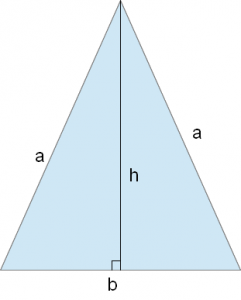
\includegraphics[height=140pt]{imagenes/triangle.png}}
	
	\end{enumerate}

\end{ejer}










\section{Logaritmos}\label{log}

En {\sage} podemos calcular logaritmos mediante \lstinline|log(x,base=b).n()|, y
se verifica que, \lstinline|b^(log(x,base=b).n())| es
aproximadamente {\tt x}, por definici\'on de logaritmo. Si no se especifica una
base los logaritmos son
naturales, neperianos, con base el n\'umero~$e$.


\begin{enumerate}
 \item Los logaritmos pueden servir para calcular el n\'umero de cifras de la
expresi\'on en base $b$ de un entero. Si 
 $b^k\le N<b^{k+1}$ vemos, tomando logaritmos en base $b$, que $k \le \log_b(N)
<
k+1$, de forma que \lstinline|k=floor(log(N,base=b).n())|. Entonces, la mayor
potencia de $b$ que aparece en la expresi\'on en base $b$ de $N$ es $b^k$ y el
n\'umero de cifras es $k+1$. Por ejemplo, podemos calcular el n\'umero de bits
necesarios para representar un entero $N$ calculando su logaritmo en base $2$.

 \item Tambi\'en podemos calcular la cifra dominante, manteniendo la notaci\'on
anterior, el coeficiente de $b^k$: 

Tenemos ahora $C\cdot b^k\le N<(C+1)b^k$, y tomando logaritmos en base $b$ otra
vez 
\[\log_b(C)+k\le \log_b(N)< \log_b(C+1)+k,\]
\noindent de forma que, restando $k$ a los tres t\'erminos y exponenciando en
base $b$, obtenemos
\[C\le b^{\log_b(N)-k}<C+1.\]

Teniendo en cuenta que $C$ es un d\'{i}gito en base $b$, 
vemos que la parte entera por defecto de  $b^{\log_b(N)-k}$ determina $C$.
 \item La utilidad de este resultado radica en que hace posible calcular la cifra dominante de un entero $N$ de la forma $a^ n$, de manera muy eficiente y  sin calcular $N$. 
 \item Ya usamos, en el ejercicio \ref{fib-log} del cap\'{\i}tulo \ref{tn1},
logaritmos para calcular el $n$ que corresponde a un n\'umero de Fibonacci $F_n$
dado.
 
\end{enumerate}


\subsection{Un problema de Gelfand}
\begin{ejer}
 
Para cada $n=1,2,3,4,\dots$ consideramos la lista formada por los d\'igitos
dominantes de $b^n$ con $b$ un d\'{\i}gito decimal excluyendo $0$ y $1$. Para
cada $n$ obtenemos una lista $L_n$  con entradas d\'{\i}gitos decimales
excluyendo el $0$:

\begin{enumerate}
 \item ?`Aparece el $9$ como cifra dominante de un $2^n$?
 \item La lista que obtenemos para $n=1$, {\tt
[2,3,4,5,6,7,8,9]} ?`vuelve a aparecer para alg\'un $n>1$? 
\item ?`Para alg\'un $n$ estar\'a la lista $L_n$ formada por $8$ repeticiones
del mismo d\'{\i}gito?
\item ?`Para alg\'un $n$ estar\'a la lista $L_n$ formada por los d\'{\i}gitos de
un n\'umero primo de ocho cifras?
 
 \item Estas preguntas, modificadas ligeramente, pueden enunciarse usando
d\'{\i}gitos en otra base $b$, y, {\itshape a priori}, deber\'{\i}a ser m\'as
f\'acil que tengan respuesta afirmativa con bases menores que $10$. Estudia las
modificaciones necesarias en los enunciados y trata de determinar si la
respuesta es afirmativa para estos enunciados modificados.
 \end{enumerate}

 Este ejercicio se puede hacer porque disponemos de una manera r\'apida, usando
logaritmos, para calcular la cifra dominante de un entero $b^n$, pero puede
ocurrir que los $n$ que buscamos con nuestro programa sean tan grandes que no
podamos llegar a verlos, o simplemente que perdamos la paciencia y paremos el
programa.

Para una soluci\'on ver la hoja 
\href{http://sage.mat.uam.es:8888/home/pub/??/}{\tt
79-APROX-gelfand.sws}.

\end{ejer}

\section{Ceros de funciones}\label{raices}


Newton encontr\'o un m\'etodo, todav\'{\i}a importante,  para obtener valores
aproximados de las soluciones de ecuaciones de la forma $F(x)=a$ sin m\'as que
suponer la funci\'on $F$ suficientemente derivable. Comenzamos estudiando el
caso particular en que la funci\'on es exponencial.

\subsection{Existencia de logaritmos}

Dado un n\'umero real $a>0$, queremos  resolver la ecuaci\'on $e^x=a$, es decir,
queremos calcular, de manera aproximada,  el logaritmo de $a$. Definimos la
funci\'on
$F_a(x):=e^x-a$, de forma que debemos ver que, para cada $a>0$ hay un n\'umero
$x$ tal que $F_a(x)=0$.

La idea es bastante simple: supongamos que $F_a(x_0)\ne 0$ y consideremos la
recta tangente a la gr\'afica de la funci\'on $F_a$ en el punto
$(x_0,F_a(x_0))=(x_0,e^{x_0}-a)$ que tiene ecuaci\'on 
\[y-(e^{x_0}-a)=(F_a)^{\prime}(x_0)(x-x_0)=e^{x_0}(x-x_0)\]
\noindent ya que la derivada de $F_a(x)$ en $x_0$ es $e^{x_0}$ (``la derivada de
la exponencial es ella misma''). La idea de Newton es que si cortamos la recta
tangente con el eje de las $X$, con ecuaci\'on $y=0$, el punto de corte puede
estar m\'as cerca de una verdadera soluci\'on de lo que estaba $x_0$. 

\begin{center}
 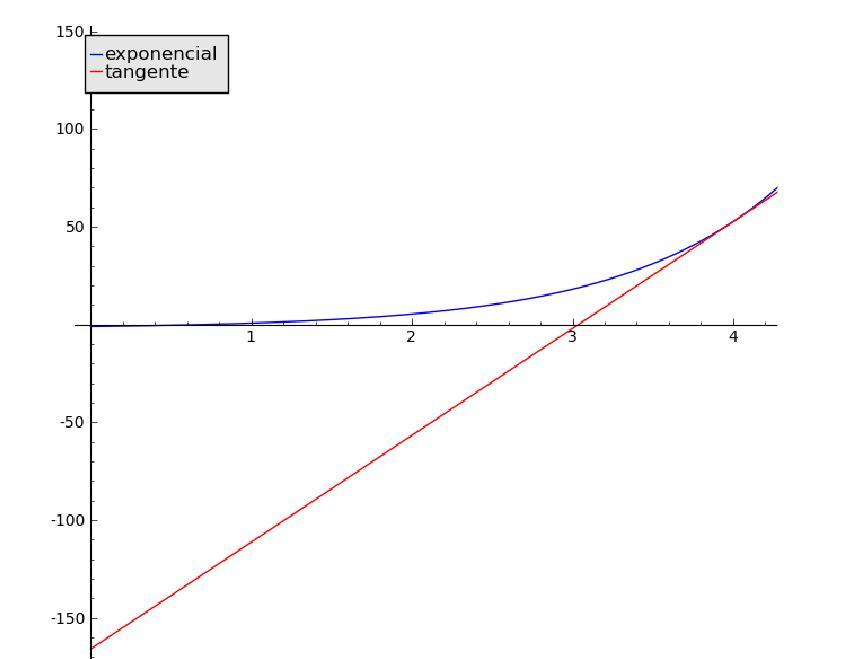
\includegraphics[scale=0.3]{imagenes/graf_exp2}
\end{center}

En la gr\'afica hemos tomado $a=2$, es decir, buscamos un $x$ tal que $e^x$
valga $2$, y empezamos con $x_0=4$ que est\'a bastante lejos de ser una
soluci\'on.  Sin embargo, la recta tangente en $(4,e^4-2)$ corta al eje de las
$X$ en un punto $(x_1,0)$ pr\'oximo a $3$,  que est\'a m\'as cerca de la
verdadera soluci\'on que vemos en la gr\'afica que ser\'a un valor bastante
cercano a cero. 


Para acercarmos m\'as a la soluci\'on bastar\'a repetir el mismo procedimiento
cambiando $x_0$ por la nueva soluci\'on aproximada~$x_1$. ?`Cu\'anto vale $x_1$?

Resolviendo el sistema formado por la ecuaci\'on de la recta tangente y la
ecuaci\'on $y=0$ obtenemos
\[x_1=x_0+\frac{e^{x_0}-a}{e^{x_0}}.\]

Definamos $T(x):= x+\frac{e^{x}-a}{e^x}$, de forma que $x_1=T(x_0)$ y la
sucesi\'on de puntos que deber\'{\i}a aproximarse a la soluci\'on es 
\[x_0,T(x_0),T(T(x_0)),T(T(T(x_0))),\dots.\]

\begin{lstlisting}[title=Método de Newton]
def Nw(x,a):
    return (x-((e^x-a)/e^x)).n()
    
def itera_hasta(ini,a,E):
    x = ini
    cont = 0
    while (abs((e^x-a).n())>E):
        x = Nw(x,a)
        cont +=1
    return x, log(a).n(), cont
    
itera_hasta(4,2,.000001)
\end{lstlisting}
\begin{Output}
	(0.693147188845376, 0.693147180559945, 7)
\end{Output}

% 
% \begin{center}
%  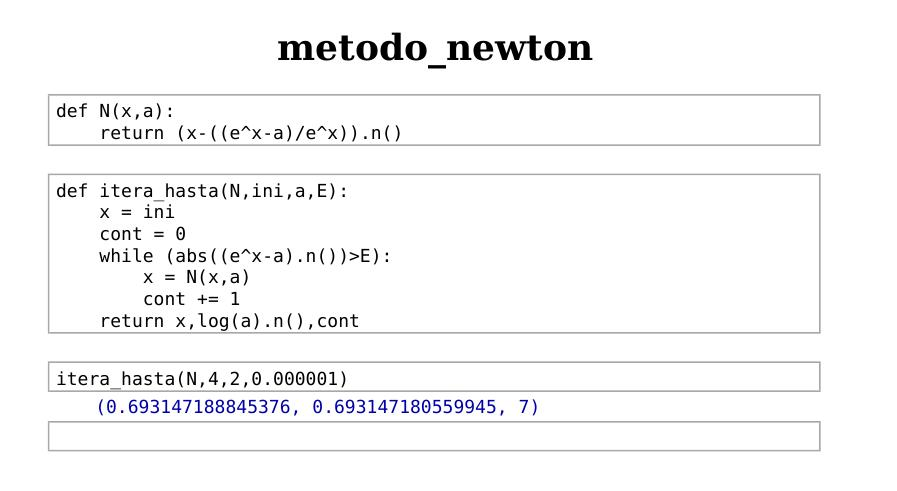
\includegraphics[scale=0.7]{imagenes/newton}
% \end{center}
% 
% ****pasar la grafica a texto*********************


Vemos que empezando en $x_0=4$ llegamos a calcular el logaritmo de $2$ con un
error menor que una millon\'esima ($E=0{.}000001$) aplicando la funci\'on
\lstinline$Nw$
siete veces,  y  tomando un valor de $E$ todav\'{\i}a m\'as peque\~no
podr\'{\i}amos conseguir una aproximaci\'on tan buena como queramos. 


Como esto podemos hacerlo para cualquier $a>0$, tenemos cierta evidencia acerca
de la existencia de un logaritmo $\log(a)$ para cada $a>0$. 


\subsection{M\'etodo de Newton}

Queremos encontar un n\'umero real $x$ tal que $F(x)=0$ y comenzamos con una
soluci\'on aproximada $x_0$.
La ecuaci\'on de la recta tangente en el punto $(x_0,F(x_0))$ es 
\[y-F(x_0)=F^{\prime}(x_0)(x-x_0),\]
que corta al eje $OX$ en $x_0-\frac{F(x_0)}{F^{\prime}(x_0)}.$ Entonces, la
transformaci\'on $T$ que debemos iterar se define como
\[T(x):=x-\frac{F(x)}{F^{\prime}(x)},\]
\noindent y esperamos que $T^n(x_0)$ se aproxime, cuando $n$ tiende a infinito, 
a un punto en el que $F$ se anula. ?`Bajo qu\'e condiciones podemos asegurar que
$T(x_0)$ es una mejor aproximaci\'on que $x_0$?

Por ejemplo, tenemos el siguiente resultado\footnote{Puede verse la
demostraci\'on en las p\'aginas 60-61 de J.Dieudonne, {\itshape C\'alculo
Infinitesimal.}}

{\itshape Sea $f$ una funci\'on continua y derivable en el intervalo real $I$,
$x_0\in I$ un punto,  y supongamos que existen constantes $C\ge 0,\ \lambda>0$
tales que 
\begin{enumerate}
 \item $\vert f(x_0)\vert \le (C/2)\lambda,$ es decir, $f$ toma valores
peque\~nos cerca de $x_0$. 
 \item Para todo par de puntos $x,y\in [x_0-C,x_0+C]\subset I$ se verifica
 \begin{enumerate}
  \item $\vert f^{\prime}(x)\vert\ge 1/\lambda,$ la derivada de $f$ no se hace
muy pr\'oxima a cero en el intervalo.
  \item $\vert f^{\prime}(x)-f^{\prime}(y)\vert\le (1/2)\lambda, $ la derivada
de $f$ no var\'{\i}a mucho en el intervalo. 
 \end{enumerate}
Entonces, existe una \'unica soluci\'on,  $\xi_0$, de la ecuaci\'on $f(x)=0$ en
el intervalo $[x_0-C,x_0+C]$ y es el l\'{\i}mite de la sucesi\'on recursiva 
\[x_{n+1}:=x_n-\frac{f(x_n)}{f^{\prime}(x_n)}.\]
\end{enumerate}
}




\subsection{Bisecci\'on}

El m\'etodo de bisecci\'on es una consecuencia del teorema de Bolzano: {\itshape
si una funci\'on continua en un intervalo $[a,b]$ verifica $f(a)\cdot f(b)<0$
entonces existe un $c\in [a,b]$ tal que $f(c)=0$. }

Para utilizarlo observamos que si el intervalo $[a,b]$ verifica la condici\'on
$f(a)\cdot f(b)<0$, entonces, salvo que $f(\frac{a+b}{2})=0$,  al menos uno uno
de los dos subintervalos, $[a,\frac{a+b}{2}]$ o $[\frac{a+b}{2},b]$, tambi\'en
la verifica. Entonces, podemos aproximarnos a $c$ subdividiendo el intervalo
hasta que su longitud  sea menor que un valor prefijado. 



\begin{ejer}
 
 Implementa el m\'etodo de bisecci\'on definiendo una funci\'on
\lstinline|subint(f,a,b)| que devuelva uno de los  subintervalos de $[a,b]$ que
verifican la condici\'on de Bolzano, y una segunda funci\'on
\lstinline|iterador(f,a,b,E)| que subdivida el intervalo hasta que la diferencia
en valor absoluto entre los extremos sea menor que \lstinline$E$, y devuelva 
el \'ultimo intervalo que ha calculado.
\end{ejer}


Este procedimiento devuelve un intervalo de longitud menor que un $E$ prefijado
y que, por el teorema de Bolzano, contiene un $c$ en el que $f(c)$ es cero. Es
de naturaleza bastante diferente al m\'etodo de Newton ya que \'unicamente
utiliza la continuidad de la funci\'on, un concepto muy posterior al de
derivada.



\section{Aproximaci\'on de funciones}
Los polinomios, que se construyen simplemente usando las cuatro operaciones
aritm\'eticas, son sin duda las funciones m\'as sencillas que se despachan. 
Resulta entonces natural tratar de usar polinomios para estudiar funciones m\'as
complejas, tratando de encontrar polinomios cuyos valores est\'en pr\'oximos a
los de la funci\'on a estudiar. 

Esto lleva, en primer lugar, a la idea de los {\itshape polinomios
interpoladores, i.e. polinomios cuyos valores en 
un  cierto n\'umero de puntos prefijados coinciden con los valores que toma la
funci\'on que estamos estudiando.}  Los polinomios interpoladores, que est\'an
forzados a coincidir con la funci\'on  en un cierto n\'umero de puntos,
tienen tendencia a alejarse bastante de la funci\'on en otros puntos, y, por
tanto, no podemos decir que sean una {\itshape buena aproximaci'on} de la
funci\'on, pero tienen algunas aplicaciones interesantes. 

Los polinomios interpoladores  ya aparecieron  como \hyperref[interp1]{ejemplo
de problema de \'algebra lineal.}

\subsection{Interpolaci\'on de Lagrange}\label{pol-int}

Un polinomio de grado $n$ tiene $n+1$ coeficientes y podemos fijar sus valores
en $n+1$ puntos distintos $x_i$. Mediante el ``m\'etodo de los coeficientes
indeterminados'', suponiendo que el polinomio buscado es
\[p(x)=a_0+a_1x+a_2x^2+\dots+a_nx^n,\]
\noindent y sustituyendo cada uno de los puntos $x_i$ e igualando al valor
prefijado en ese punto $y_i$, obtenemos un sistema lineal %inhomog\'eneo 
de ecuaciones, $n+1$ ecuaciones con $n+1$ inc\'ognitas, cuya matriz es una 
\href{http://en.wikipedia.org/wiki/Vandermonde_matrix}{matriz de Vandermonde}
con determinante siempre no nulo si los $x_i$ son distintos entre s\'{\i}.

Entonces, el polinomio interpolador existe y es la \'unica soluci\'on del
sistema lineal obtenido. En la pr\'actica no resolvemos el sistema lineal ya que
existe una f\'ormula, debida a Lagrange, que nos da directamente el
\href{http://en.wikipedia.org/wiki/Lagrange_polynomial}{polinomio
interpolador.}

\par
\medskip
\par

El polinomio interpolador se utiliza para estudiar, por el m\'etodo de
Kronecker, la \hyperref[kron]{irreducibilidad de polinomios} con coeficientes
enteros.  Tambi\'en lo hemos usado para obtener
\hyperref[ej-SumaCubos]{f\'ormulas para las sumas de potencias}
\[p(n,k):=1^k+2^k+3^k+\dots+n^k,\]
\noindent ya que una vez que sabemos, debido a que la suma es muy parecida a la
integral definida
\[\int_1^n x^k dx,\]
 \noindent que el resultado debe ser un polinomio de grado $k+1$, es f\'acil
obtener sus coeficientes por interpolaci\'on en $i=1,2,3,\dots,k+1$ ya que es
f\'acil calcular directamente los valores $p(i,k)$. 

\subsection{Interpolaci\'on de Newton y polinomio de Taylor}\label{dif-div}



Dados $n+1$ valores distintos $x_0,\dots,x_n$ distintos, y una función $f(x)$, 
se definen, recursivamente, las {\sc diferencias divididas}:
\begin{align*}
f[x_0,x_1] &=\frac{f(x_1)-f(x_0)}{x_1-x_0}
&&\text{ si }n=1\\
f[x_0,x_1,\dots,x_n]&=
\frac
{f[x_1,\dots,x_n]-f[x_0,x_1,\dots,x_{n-1}]}
{x_n-x_0}&&\text{ para }n\ge2\,.
\end{align*}
Se tiene el siguiente:
\begin{tma}\label{difgral}
Sean $(x_0,f(x_0))$, $(x_1,f(x_1))$, $\dots$, $(x_n,f(x_n))$, $n+1$
puntos distintos de la gráfica de $f$. El polinomio interpolador de
grado $n$ que pasa por estos $n+1$ puntos es
\begin{align*}
P_n(x) & =f(x_0)+\sum_{k=1}^n f[x_0,\dots,x_k]\prod_{i=0}^{k-1}(x-x_{i})
\\
&=
f(x_0)+f[x_0,x_1](x-x_0)
+f[x_0,x_1,x_2](x-x_0)(x-x_1)+\dots\\
&  \quad\dots\dots\,+
f[x_0,x_1,\dots,x_n](x-x_0)(x-x_1)\cdot
\dots\cdot(x-x_{n-1}).
\end{align*}
\end{tma}

El polinomio interpolador de Newton es el mismo que el de Lagrange, a fin de
cuentas el polinomio interpolador es \'unico, pero expresado en la base del
espacio de polinomios de grado $\le n$ dada por los polinomios
$\prod_{i=0}^{k-1}(x-x_{i})$ mientras que el de Lagrange est\'a expresado en la
base de monomios $x^k$.



\begin{ejer}
 Encontrar, utilizando la forma de Newton, el polinomio de menor grado cuya
gráfica pasa por los puntos
 $$
 (-2, 26), (-1, 4), (1, 8), (2, -2)\,.
 $$
 
Comparar el método utilizado con el anterior, de coeficientes indeterminados.
\end{ejer}


El aspecto quiz\'a m\'as interesante del polinomio interpolador de Newton es que
se trata de una versi\'on discreta del \hyperref[taylor]{polinomio de Taylor}: cuando todos los
puntos $x_i$ se hacen coincidir en un \'unico punto $z$ el polinomio
interpolador nos da el polinomio de Taylor. 






Sabemos que la derivada en $x_0$ permite aproximar una funci\'on $f(x)$, 
derivable en $x_0$, mediante una funci\'on lineal 
\begin{equation}\label{tang}
f(x)=f(x_0)+f^{\prime}(x_0)(x-x_0)+\dots.
\end{equation}
De la misma forma, el polinomio de Taylor permite aproximar una funci\'on,
derivable $k$ veces, en la forma
\[f(x)=f(x_0)+f^{\prime}(x_0)(x-x_0)+\frac{f^{\prime\prime}(x_0)}{2!}
(x-x_0)^2+\dots+ \frac{f^{(k)}(x_0)}{k!}(x-x_0)^k+\dots\]

Estas aproximaciones de una funci\'on suficientemente derivable mediante un
polinomio son {\itshape locales}: \'unicamente son v\'alidas para $x$ muy
pr\'oximo a $x_0$, pero en general no valen lejos de $x_0$. Por ejemplo, la
gr\'afica de la funci\'on lineal en (\ref{tang}) es la recta tangente, en $x_0$,
 a la gr\'afica de la funci\'on $f$, y lejos de $x_0$ puede estar muy separada
de la gr\'afica de $f$.
\subsection{{\tt find\_fit}}
Mediante la t\'ecnica de interpolaci\'on conseguimos un polinomio de grado
m\'{\i}nimo tal que su gr\'afica pasa exactamente por un conjunto dado de
puntos del plano. Esta condici\'on es demasiado restrictiva y fuerza en
ocasiones al polinomio interpolador a tener un comportamiento extra\~no.


Podemos relajarla buscando una funci\'on m\'as sencilla, por ejemplo una recta,
que pase {\itshape lo m\'as cerca que sea posible} de todos los puntos, pero
sin pasar necesariamente por ninguno de ellos. Se llama a esta t\'ecnica
{\itshape regresi\'on}, y consiste, en resumen, en lo siguiente:

\begin{enumerate}
 \item Representamos gr\'aficamente los puntos en el plano,
\lstinline|points(L)|, con $L$ la lista de $2$-tuplas formada por las
coordenadas, y tratamos de {\itshape ver la forma de la curva que mejor se
adapta}. Esto nos permite proponer un {\itshape modelo} $f(x,a_1,a_2,\dots)$ con
$x$ la variable independiente y los $a_i$ par\'ametros del modelo. 
\item Si los puntos son $(x_i,y_i)$ definimos los residuos
\[r_i(a_1,a_2,\dots):=y_i-f(x_i,a_1,a_2,\dots),\]
\noindent que son funci\'on de los par\'ametros $a_i$.
\item Definimos el {\itshape error cuadr\'atico medio} como 
\[S(a_1,a_2,\dots):=\sum r_i(a_1,a_2,\dots)^2.\]
Al elevar al cuadrado los residuos eliminamos su signo, de forma que todos
contribuyen incrementando $S(a_1,a_2,\dots).$
\item Minimizamos la funci\'on $S((a_1,a_2,\dots)$, es decir, calculamos los
valores de los par\'ametros que hacen m\'{\i}nimo el error cuadr\'atico medio.
Los valores que minimizan son los que declaramos {\itshape valores \'optimos}
para este problema. 
\end{enumerate}

Esta idea tiene muchas variantes, y puedes leer sobre ella en 
esta p\'agina de la 
\href{http://en.wikipedia.org/wiki/Non-linear_least_squares}{Wikipedia.}

En {\sage} se puede ajustar un modelo a una lista de puntos mediante, por
ejemplo,
\begin{lstlisting}
 var('a b')
 modelo(x)=a*x+b
 find_fit(L,modelo)
\end{lstlisting}
\noindent que nos devuelve los valores de los par\'ametros $a,b$ que hacen
m\'{\i}nimo el error cuadr\'atico medio. En este caso el modelo es lineal, pero
podemos definirlo mediante una funci\'on arbitraria.

En ocasiones el valor de alguno de los par\'ametros es muy peque\~no, y debemos
sospechar que el modelo correcto no depende de ese par\'ametro. Cambiamos la
definici\'on del modelo y comparamos, al menos mediante gr\'aficas, los dos
ajustes.


Esta instrucci\'on es muy \'util, y veremos ejemplos a lo largo del curso, para
tratar de averiguar la forma de una  funci\'on desconocida cuando hemos
calculado en el ordenador sus valores para un cierto n\'umero de valores de su
variable independiente. Un primer ejemplo aparece al resolver el tercer
ejercicio en la \hyperref[ejer-7]{lista al final de este cap\'{\i}tulo.} 

\subsection{Otros {\tt find\_...}}

Aparte de {\tt find\_fit}, {\sage} dispone de, al menos otras $3$ instrucciones
que comienzan en la forma {\tt find\_...}:

\begin{enumerate}
 \item {\tt find\_local\_maximum(f,a,b)} ({\tt find\_local\_minimum(f,a,b)})
devuelve un m\'aximo ( m\'{\i}nimo local) de la funci\'on $f$ en el intervalo
$[a,b]$. El m\'aximo (m\'{\i}nimo) devuelto no tiene que ser el mayor (menor)
de los m\'aximos (m\'{\i}nimos) locales de la funci\'on en el intervalo.
 
 
 \item {\tt find\_root(f,a,b)} devuelve un cero, aproximado,  de la funci\'on
$f$ en el intervalo $[a,b]$. No admite precisi\'on arbitraria ni devuelve todos
los ceros. Es posible crear un programa que subdivida el intervalo  en
subintervalos muy peque\~nos y aplique la funci\'on en cada uno de ellos, en la
esperanza de que haya un \'unico cero en cada uno de los subintervalos.
 
 
 
 
\end{enumerate}




\subsection{Aproximaci\'on global}

Un problema diferente, pero muy interesante, es la {\itshape aproximaci\'on
global} a una funci\'on dada: supongamos que $f(x)$ sea una funci\'on continua
definida en el intervalo $[0,1]$ de la recta real. Queremos encontrar una
familia de polinomios $B_{n,f}(x)$ que se ``aproximen'' a $f$ en todo el
intervalo
$[0,1]$ cuando $n$ crece. 

 Los polinomios interpoladores, que est\'an forzados a
coincidir con la funci\'on $f$ en un cierto n\'umero de puntos, tienen
tendencia a alejarse bastante de la funci\'on en otros puntos. Entonces no
resuelven el {\itshape problema de aproximaci\'on global.}



Una soluci\'on son los {\itshape polinomios de Bernstein}, definidos en la
forma 
\[B_{n,f}(x):=\sum_{p=0}^{p=n} \binom{n}{p}f(p/n)(1-x)^{n-p}x^p.\]

?`Cu\'al puede ser la idea de esta definici\'on? Si $f(x)$ es constante e igual
a $1$, el polinomio $B_{n,f}(x)$ es, gracias a la f\'ormula del binomio de
Newton, igual a $(1-x+x)^n=1^n=1$. Entonces para una funci\'on constante se
obtiene que todos los polinomios de Bernstein son constantes e iguales a la
funci\'on. 

Por otra parte, cada uno de sus sumandos
$b_{n,p}(x):=\binom{n}{p}(1-x)^{n-p}x^p$ es un polinomio de grado $n$ y todos
juntos forman una base, la {\itshape base de Bernstein},   del espacio vectorial
de polinomios de grado $\le n$, de forma que $B_{n,f}(x)$ viene definido como
una combinaci\'on lineal de los polinomios de la base con ciertos coeficientes
que dependen de $f$. 

Antes de continuar representamos los polinomios $b(5,p)$ mediante la
instrucci\'on \lstinline|sum([plot(b(5,p),0,1) for p in srange(6)])| que produce
\begin{center}
 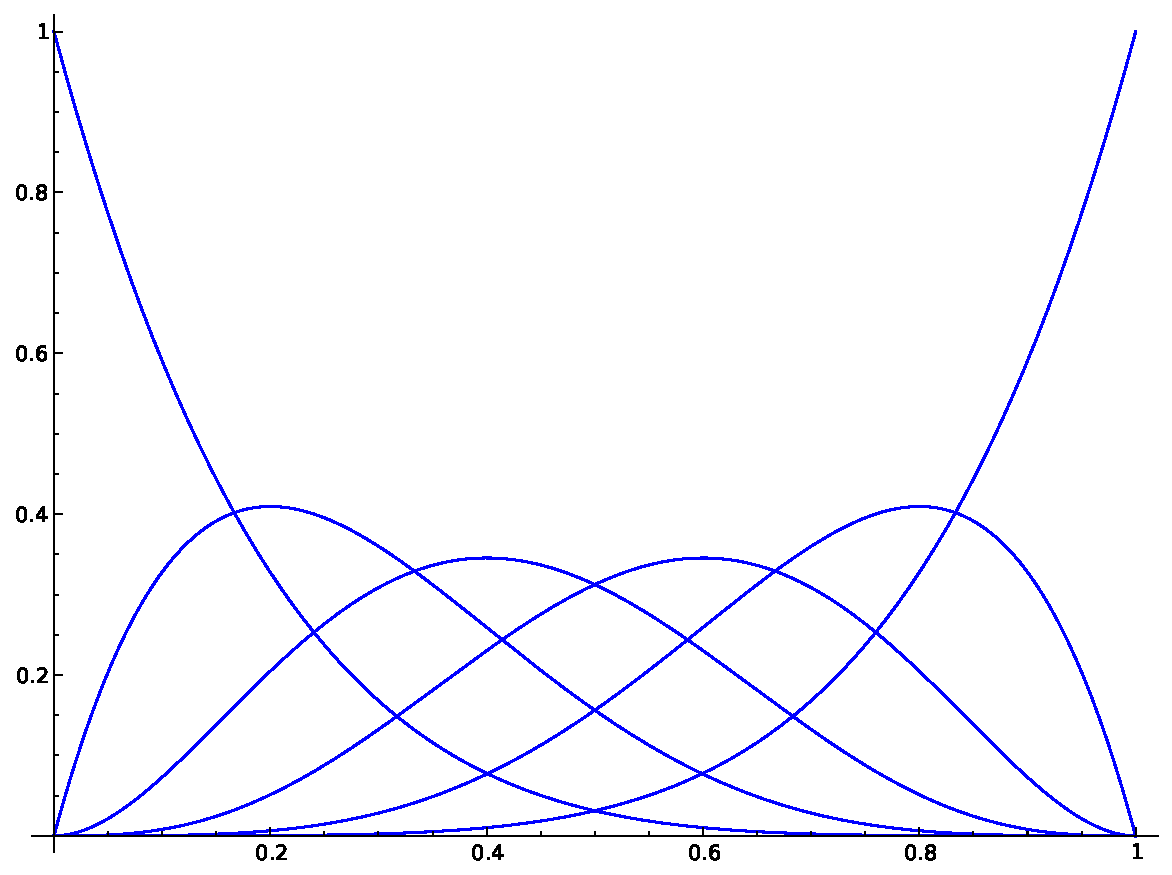
\includegraphics[scale=0.24]{bernstein-p}
\end{center}
\noindent y vemos que el polinomio $b(5,p)$ tiene su m\'aximo, m\'as o menos, 
en el punto $x=p/5$. Como luego estamos tomando como coeficiente de $b(5,p)$ el
valor de $f$ en $p/n$, podemos concluir que lo que hace la f\'ormula que define
$B_{n,f}(x)$ es usar, cerca de $p/n$, la aproximaci\'on  $f(p/n)b_{n,p}(x)$ y
luego sumar todas esas aproximaciones. Cuando $n$ crece usamos muchos m\'as
valores $f(p/n)$ y, se puede demostrar\footnote{Verlas las p\'aginas 166-167 de
J.Dieudonne, {\itshape C\'alculo
Infinitesimal.}}  , que el polinomio $B_n(x)$
se aproxima
globalmente a $f(x).$

\

\begin{ejer}


\begin{enumerate}
  \item Define una funci\'on de {\sage} que dependa de un entero $n$ y una
funci\'on $f$ y devuelva $B_{n,f}(x).$ 

\item Experimenta, mediante gr\'aficas,  con diversas funciones $f$, continuas
en $[0,1]$ y sus aproximaciones. Por ejemplo, podemos tomar
$f(x)=\mathrm{sen}(2\pi x)$,
$f(x)=\mathrm{sen}(4\pi x)$, etc.

\item Trata dar una definici\'on razonable que precise en qu\'e sentido
$B_{n,f}(x)$ aproxima a $f(x)$ globalmente en el intervalo $[0,1].$

\item Dado que la aproximaci\'on de $B_{n,f}(x)$ a $f(x)$ es global, podr\'{\i}a
ser razonable calcular aproximadamente la integral 
\[\int_0^1 f(x)dx \text{ mediante }  \int_0^1 B_{n,f}(x)dx, \]
con $n$ suficientemente grande. ?`Qu\'e opinas de este m\'etodo?
\end{enumerate}
\end{ejer}

\section{Ejercicios}\label{ejer-7}
\begin{ejer}
 
 El n\'umero $e$ se puede obtener, entre otras, de una de las siguientes maneras
\begin{enumerate}
\item     \[\lim_{n\to \infty}(1+\frac{1}{n})^n.\]
\item     \[\sum_{n=0}^{n=\infty}\frac{1}{n!}.\]
 \item    \[lim_{n\to \infty}
\frac{n^n}{(n-1)^{n-1}}-\frac{(n-1)^{n-1}}{(n-2)^{n-2}};
n>2.\]
\end{enumerate}
Este ejercicio trata de calcular valores aproximados del n\'umero $e$ usando
cada una de las expresiones anteriores y de estudiar el {\itshape coste
computacional} de los c\'alculos, \hyperref[time]{usando},  por ejemplo. 
\lstinline|time| o \lstinline|timeit|, tratando de responder a la pregunta
natural: ¿Cu\'al es el mejor m\'etodo?

\end{ejer}


\begin{ejer}
 
 Consideramos la serie \footnote{Propuesta en J. Borwein, D. Bailey, R.
Girgensohn, {\itshape Experimentation in Mathematics}, (2004), Ed. A K Peters.} 
 \[\sum_{n=1}^{n=\infty} \frac{floor(n\cdot tanh(\pi))}{10^n},\]
 \noindent con {\tt floor} la funci\'on {\itshape parte entera por defecto} y
{\tt tanh} la tangente hiperb\'olica.

{\sc Comprueba} que las $268$ primeras cifras decimales  de la suma de la serie
coinciden con las primeras $268$ cifras de la fracci\'on $1/81,$ pero las cifras que podemos calcular a continuaci\'on ya no coinciden.  

La explicaci\'on, indicada en el libro citado en la nota a pie de p\'agina, es que la tangente hiperb\'olica
de $\pi$ est\'a muy pr\'oxima a $1$ ($0{.}99<tanh(\pi)<1$) de forma que el
numerador de los sumandos de la serie es, para muchos $n$ igual a $n-1$, y
ahora se tiene 
\[\sum_{n=1}^{n=\infty} \frac{n-1}{10^n}=\frac{1}{81}.\]

Este ejemplo ilustra claramente el peligro que corremos al suponer que algo que
hemos {\itshape comprobado experimentalmente}, hasta el punto  que nos ha
permitido el {\itshape hardware} o {\itshape software} del ordenador, es una
verdad matem\'atica. 
 
\end{ejer}


\begin{ejer} 

({\sc Aproximaci\'on de Stirling}) Queremos obtener una
estimaci\'on del valor del factorial de $n$ que sea lo m\'as precisa posible
para $n$ muy grande. Esta estimaci\'on tiene gran cantidad de usos, y es muy
importante, por ejemplo, en Mec\'anica Estad\'{\i}stica,  que es el estudio de
sistemas de part\'{\i}culas, gases , s\'olidos, etc., con un n\'umero de
part\'{\i}culas del orden del n\'umero de Avogadro  $6\cdot 10^23.$
 
 En este ejercicio combinamos ideas te\'oricas con c\'alculos en ordenador para
dar una {\itshape justificaci\'on experimental} de la aproximaci\'on de
Stirling.

\begin{enumerate}
 \item Comenzamos tomando logaritmos neperianos (naturales):
 
 \[log(n!)=log(1)+log(2)+log(3)+\dots+log(n),\]
 \noindent y esta suma se puede calcular aproximadamente, vi\'endola como una
suma de Riemann, como la  integral 
\[\int_1^n log(x)dx=n\cdot log(n)-n+1.\]

\item Nos quedamos con la aproximaci\'on $log(n!)=n\cdot log(n)-n$, o su
equivalente exponenciando
\[n!=n^n\cdot e^{-n}=\frac{n^n}{e^n},\]
\noindent que nos dice que, en una no muy buena aproximaci\'on, el exceso que
se obtiene al calcular $n^n=n\cdot n\cdot n\dots \text{ $n$ veces }\dots n\cdot
n$ cuando en realidad queremos $n!=1\cdot 2\cdot 3\dots (n-1)\cdot n$ se
compensa, en gran medida,  dividiendo entre $e^n$.

\item Definimos la funci\'on 
\[F(n):=\frac{n!}{n^n\cdot e^{-n}},\]
\noindent y usamos {\sage} para calcular un gran n\'umero de valores de $F(n)$,
por ejemplo $F(n)$ para $n$ entre $1$ y $50000$.

\item Obtenemos una representaci\'on gr\'afica de los $50000$ puntos obtenidos
en el apartado anterior y proponemos un modelo razonable para ajustar una
funci\'on a los puntos usando \lstinline|find_fit|.
\label{stirling}
\item Tratamos de identificar el par\'ametro del modelo, es razonable en este
caso, vista la gr\'afica,  suponer que depende de un \'unico par\'ametro, usando
la
\href{https://oeis.org/}{{\itshape  Enciclopedia de sucesiones de enteros}}: en
la p\'agina de entrada podemos escribir las cifras decimales del valor obtenido
para el par\'ametro, separadas por comas, y nos devuelve una lista de
cosntantes matem\'aticas en las que aparece de alguna manera esa sucesi\'on de
cifras. 

La Enciclopedia permite identificar sucesiones  de enteros, no
s\'olo de d\'igitos, como por ejemplo, la sucesi\'on de Fibonacci y es
enormemente \'util al realizar {\itshape experimentos matem\'aticos.}
\end{enumerate}


 
 
 
 \end{ejer}